\documentclass[a4,12pt]{report}
\usepackage[Bjornstrup]{fncychap}
\usepackage{graphicx}
\usepackage{epsf}
\usepackage{a4}
\usepackage{fancyhdr}
\usepackage{setspace}
\usepackage{amsmath}
\usepackage{amsfonts}
\usepackage{amssymb}
\usepackage{enumerate}

\usepackage{caption}
\usepackage{epsfig}
\usepackage{subfigure}
\usepackage{colortbl}
\usepackage{color}
\usepackage{rotate}
\usepackage{rotating}
\usepackage{amsthm}
\usepackage{booktabs}
\usepackage{slashbox}



\usepackage{relsize}
\usepackage{fancyvrb}
\usepackage[colorlinks=false]{hyperref}




\usepackage{url}
\usepackage{arabtex}

\usepackage{utf8}
\setarab
\fullvocalize
\transtrue
\arabtrue


%\newcommand{\CharCodeIn}[1]{`\CodeIn{#1}'}
\newcommand{\CodeIn}[1]{{\small\texttt{#1}}}
\newcommand{\frl}[1]{\fbox{\RL{#1}}} 
\newcommand{\noArRL}[1]{\arabfalse\RL{#1}\arabtrue} 
\newcommand{\noTrRL}[1]{\transfalse\RL{#1}\transtrue}
\newcommand{\noTrnoVocRL}[1]{\transfalse\novocalize\noTrRL{#1}\vocalize\transtrue}  
\newcommand{\noVocRL}[1]{\transtrue\novocalize\RL{#1}\vocalize}  

\newcommand{\X}{\cellcolor[gray]{0.5}}
\newcommand{\x}{\cellcolor[gray]{0.8}}

%Header and Footer
\fancyhead{} \fancyhead[LO,RE]{\scriptsize\sc\leftmark}
%\fancyhead[R]{Jad Makhlouta}
\fancyfoot[l]{ \scriptsize \textit{AUB, Spring 2010-2011}}
\fancyfoot[R]{ \scriptsize \textit{ Thesis Proposal Report}}


%-------BEGIN----------------------------------------------------
\begin{document}


%----------------Report Cover--------------------------------------------------
%\documentclass[11pt,a4paper]{letter}
\usepackage{graphicx}
\usepackage{multirow}

\oddsidemargin -0.25in
\evensidemargin -0.25in
\topmargin -1in
%\topsep 0in
\textheight 10.25in
\textwidth 6.75in
%\parskip 6pt
\longindentation 0.5\textwidth
\parindent 0.4in

\begin{document}

\address{
    \begin{tabular}{p{4.2cm}p{6cm}r}
%    \multirow{3}{*} {
%    \includegraphics[width=4cm]{../AUB-concise-logo-color.jpg} } & &
& & Fadi A. Zaraket \\
& & AUB Faculty of Eng. \& Arch. \\
& & ECE Department \\
%& P.O. Box: 11-0236\\
%& Riad El-Solh, Beirut 1107 2020\\
%& Beirut, Lebanon\\
& & Tel: (+961) 1 350 000, ext: 3484  \\ \hline
& & Email: {\tt fadi.zaraket@aub.edu.lb} \\
\end{tabular}
}

\begin{letter}{}

\signature{Fadi A. Zaraket \\ Assistant Professor
  of Electrical and Computer Engineering}


\opening{Dear concerned at NLE,}

We appreciate your consideration of our submission entitled {\em Sarf: Application Customizable Efficient Arabic Morphological Analyzer}. 
The paper describes an Arabic morphological analyzer that has been used effectively and efficiently in several Arabic NLP 
applications for information extraction from Arabic text. 
The paper describes the contributions of Sarf as compared with existing work. 
Sarf provides application customizable analysis through an API that allows the NLP application developer to control and refine the 
analysis on the fly. 
Sarf refines the lexicons of existing analyzers, reduces the required size and maintenance by using agglutinative and fusional concatenation rules and solves morphological feature inconsistencies in the existing analyzers. 
Sarf also solves the token segmentation problem which is a hindrance to machine learning with current analyzers. 

We look forward for NLE to consider our submission as Sarf bridges the gap between computational linguistics and practical applications, 
provides an efficient engineering implementation for the Arabic morphological analysis problem, and is similar to 
morphological analyzers and lexical resources for other semitic languages such as Hebrew that NLE published before. 


\closing{Best regards,
    \\~
}
\vspace{-2in}

\end{letter}

\end{document}



\end{document}

\begin{titlepage}
%\vspace{1cm}
\begin{center}

% \vspace{1cm}

\large{Department of Electrical and Computer Engineering\\
Faculty of Engineering and Architecture \\
American University of Beirut\\}
\vspace{3cm}
%\begin{figure}[h]
%    \begin{center}
%       \includegraphics[scale=0.25]{Fig/aublogo.eps}
%    \end{center}
%\end{figure}
 \LARGE \textbf{Application-Specific Arabic Morphological Analyzer and \\Automatic Hadith Authentication\\}
\vspace{1.5cm}
\LARGE {Thesis Proposal \\ Spring 2010-2011}\\
\end{center}
\vspace{3.5cm}
\begin{tabbing}



Submitted by: \quad\quad \quad \quad \=Jad Makhlouta, 200700856 \\
\\
Thesis Supervisor:  \> Dr. Fadi Zaraket \\

Committee Member: \> Dr. Hasan Artail  \\

Committee Member:  \> Dr. Ibrahim Abou Faycal \\


\\
\\
\\
Submitted on: \> \today
\end{tabbing}
\end{titlepage}


% Select arabic numbering style
\pagestyle{fancy}
 \pagenumbering{arabic}
\setcounter{page}{1}

\begin{abstract}
Text Mining 
%can be considered as a subfield of both Natural Language Processing (NLP) and Data Mining.
is interested in automatically extracting useful information and relations from text documents.
%Extracted information is hard to discover manually or previously unknown
%Natural Language Processing applications perform 
%to discover useful information that is otherwise unknown.
The complexity of natural languages introduces interesting challenges 
to automatic analysis of underlying textual data.
Morphological analysis is key to many Natural Language Processing Applications.
General morphological analyzers such as Buckwalter and ElixirFM 
generate all morphological solutions.
However, this exhaustive enumeration may not be needed or appropriate for the
application at hand.
We propose developing Sarf, an Arabic application-specific morphological analyzer whose functionality can be customized 
based on the specific needs of the application. 
%This flexibility has been motivated by 
%the broad spectrum of text mining applications, each with its specific characteristics and corpora, which
%necessitate a special treatment.
Sarf encodes its lexicon into a non-deterministic composition of three finite automata.
It also solves the issue of `run-on' words, supports disambiguation using diacritics, 
handles multi-word expressions and performs online tokenization.
In our thesis, we will use Sarf to solve two useful Natural Language Processing applications: 
(1) the extraction of time entities from Arabic documents, and 
(2) the automation of the process of hadith authentication.

\end{abstract}

\chapter{Introduction}
\label{s:intro}

The world we live in overwhelms us with electronic data. There is an ever-increasing gap between the amount
of information available and our ability to understand and analyze it. ``Omnipresent computers make
it too easy to save things that previously we would have trashed. Inexpensive disks
and online storage make it too easy to postpone decisions about what to do with all
this stuff -- we simply get more memory and keep it all.''~\cite{Witten:11}
This explosion in available data has motivated the automation of the task 
of extracting information of interest for a certain usage. 
Manual extraction is practically unfeasible due to
our limited precious time recourses compared to the magnitude of the task.
In addition, it was shown that automatic methods have been able to discover previously unknown 
information through relating separate datasets~\cite{JNi06}.

%Consequently, \textit{Data Mining} as a field of study emerged
%as an attempt to tackle this problem which is manually unfeasible.
%Data Mining in general is defined as the task of `extraction of interesting 
%(non-trivial, implicit, previously unknown and potentially useful) patterns 
%or knowledge from huge amounts of data'~\cite{Witten:00}.

Clearly, a small percentage of the data available worldwide 
is stored in databases in structured form; instead, the greater amount of information is available in the 
form of electronic text files and documents such as news articles, publications, governmental records, etc. ...
Even old paper documents are being ported to digital form to facilitate their use. 
Text Mining emerged as an attempt to automate the extraction of interesting, 
previously unknown and potentially useful information
from the huge amounts of text documents~\cite{Witten:08}.
Information Extraction (IE) from natural languages, however, is challenged
by the difficulty of getting structured 
entities from the underlying unstructured textual data.

%Information Extraction (IE) from Natural Language Texts has always been an important 
%problem in Data mining. What distinguishes text mining from the 
%other subfields of data mining is mainly due to the challenge of getting structured 
%entities from the underlying unstructured textual data. Clearly, a small percentage of the data available worldwide 
%is stored in databases in structured form; instead the greater amount of information is available in the 
%form of electronic text files and documents such as news articles, publications, governmental records, etc. ...
%Even old paper documents are being ported to digital form to facilitate their use. 

Natural Language Processing (NLP)
as a field of research is interested in achieving a computational model of the language
and understanding its underlying meaning~\cite{sharp:01}. It is known that this task
is very complex and possibly not completely achievable. However, in most applications it 
is not needed to grasp the whole meaning of the text but to extract some useful entities.
This Information Extraction(IE) problem can be performed through some statistical approaches 
and/or partial NLP techniques.

A subproblem of NLP is morphology.
Morphological analyzers%~\cite{Sughaiyer:04}
are interested in understanding the internal structure of a word;
It considers words as being composed of 
several {\em morphemes}. 
A morpheme is a {\em stem} or an {\em affix}.
An affix is a {\em prefix, suffix,} or an {\em infix}.
Prefixes and suffixes are attached to the beginning and end of the word respectively; 
while infixes introduce changes in the stem itself. 
Morphological analyzers have been extensively used as building blocks 
in many text mining applications~\cite{Sou07}.  In Arabic, many morphological analyzers exist including:  
Buckwalter~\cite{Buckwalter:02},
Beesley~\cite{Beesley:01},
SAMA ~\cite{Kulick:10},
ElixirFM~\cite{Otakar:07}, 
AMIRA~\cite{Diab:07,Benajiba:07},
MAGEAD~\cite{Habash:05}, 
and MADA+TOKAN~\cite{Habash:09}.
%Arabic however has distinctive characteristics that
%complicate its analysis; and consequently, much remains to be performed in the field.

In this thesis, we propose to develop Sarf, an application-specific 
morphological analyzer for the Arabic language 
which is capable of benefiting
from the specific characteristics of the application at hand. 
In addition, it supports disambiguation using diacritics and 
handles `run-on' words. We also propose to use Sarf to solve two interesting .
text mining applications: time entity extraction and hadith authentication.

\section{Applications of Text Mining}
\label{sec:Applications}

%Text Mining has gained much interest lately especially due to its wide range of applications.
%However, these applications have substantially differing corpora (terminology, 
%sentence structure, etc...). In this section, we present some of the 
%previously explored applications of text mining.
%
%Research in text mining started in the mid 1980s when Swanson 
%realized that slicing and combining seemingly unrelated medical 
%articles led to the discovery of new 
%hypotheses~\cite{JNi06}. 
%Lately we saw applications of text mining in the advertisement, 
%political campaigning, and other businesses.

Research in text mining started in the mid 1980s when Swanson 
realized that slicing and combining seemingly unrelated medical 
articles led to the discovery of new 
hypotheses~\cite{JNi06}. 
Text Mining has gained much interest lately due to its wide range of applications,
including its use in the areas of advertisement, 
political campaigning, and other businesses.
However, these applications have substantially differing corpora (terminology, 
sentence structure, etc...). In this section, we present some of the 
previously explored applications of text mining.

\subsection{Sentiment Analysis} 
	This field -- also known as Opinion Mining' -- attempts classifying the polarity of sentiments of people 
	or even their emotional state ~\cite{Pang:08}. The inputs for such analyzers include product and movie reviews, 
	Internet blogs, electronic social networks and possibly newspapers. Early research was conducted on review sites
	to automate the task classifying whether the review was positive and negative. Consequently, users can get concise helpful
	sentiment summaries about the product, movie, etc...~\cite{Pang:02, Turney:02}. Such abilities motivated research targeting 
	the following applications:
	\subsubsection{Marketing Applications} 
		The strength of blogs in disseminating opinions is a two-edged sword that can 
		``make or break a company's reputation''~\cite{hoffman:08a}. Consequently, analyzing customers' opinions as portrayed 
		on online discussion forums should be detected as soon as possible. This input is vital in the company's policy for its
		reputation management. It can accordingly take actions to retain current customers, attract new ones and win back former 
		customers~\cite{hoffman:08b}. Sentiment Mining has also been used to predict customer churns~\cite{marketing:07,marketing:08}
		to take appropriate actions. It can help also in producing more effective advertisements based on the interests of the market.
	\subsubsection{Political Applications} 
		Political experts and analysts can benefit also. Since opinions extracted from textual data 
		can reveal much even without the need of performing any explicit surveys. According to ~\cite{Gryc:10}, it ``opens up many avenues
		for more accurate and naturalistic large-scale political analysis.'' Some research has been performed on classifying and predicting
		political inclinations~\cite{Durant:07, Yu:08}. This field can help political leaders to better understand the views of their people 
		and possibly perform better campaigns.
		
\subsection{Academic Applications} 
	In scientific disciplines where written papers and publications contain technical information, the need to retrieve
	specific information that a user needs, aids in \textbf{\em developing advanced search engines}. 
	Text mining plays a great role toward this end through the following:
	\subsubsection{Text Summarization} 
		When an application is interested in mining a text for the most important and informative portions,
		the application is considered to be tackling the field of `Text Summarization'. Summaries may have different forms such as being 
		a group of representative words, to a coherent abstraction of the text in novel terms and phrases that capture its main meaning. 
		The main motivation
		for such a research is to enhance search engines. By capturing the most informative concepts in a document, it aids determining a 
		better metric for a document's relevance to a search query. It also helps search engines display a shortened preview of the document for returned
		results. This reduces the overwhelming amount of information a user needs to read before deciding weather the whole document deserves
		comprehensive study. It is also helpful when the editorial staff of a magazine or newspaper need to present an article in the limited space.
		Similarly, summarization is vital when the content of 
		news articles needs to be dramatically shortened to be sent in an SMS form to subscribed PDA users. 
		Useful surveys of current research on text Summarization can be
		found in ~\cite{Radev:02,Das:07}.
	\subsubsection{Text Categorization and Clustering} 
		In many cases, it is very useful to be able to search for documents by theme, topic, domain, etc...
		This ability is achieved if documents can be automatically clustered into different categories over which a user can search. It has been also 
		proposed to cluster documents based on biographical data~\cite{Kostoff:99}. Technically speaking the difference between Categorization and
		Clustering is that the former organizes documents into predefined categories where in the latter the categories arise from the document content
		themselves~\cite{sharp:01}. Many approaches exist in this field as described in~\cite{Berry:03, Aas:99, MUNTEANU:05}.
		\begin{enumerate}
		\item \textbf{Email Classification:} It is noteworthy to mention that it is text categorization can be used for emails 
			-- such as urgent, work, friends, spam, etc... Consequently, it can be used for spam detection and email 
			filtering~\cite{Mock:01,bekkerman:04}.
		\item \textbf{Parental Control:} It has also been proposed to use categorization for parental control by
			automatically detecting inappropriate content for their children~\cite{Kontostathis:09}.
		\end{enumerate}
	\subsubsection{Entity Extraction:} Named Entity Extraction/Recognition (NER) targets being able to detect phrases that convey some general concept
		and/or belong to a predefined set of categories such as persons, places, time, etc... It has been argued that having the luxury of searching
		for entities enhances search abilities instead of being restricted to a list of words appearing in a text~\cite{basis:06}. 
		It seems that humans think of their
		queries in terms of entities/concepts and then try translating them to some list of words which are most likely to appear in a document that
		is relevant to their search query. In general, a user does not ``know all the search terms that will return all instances of the desired
		information''~\cite{basis:06}. A survey of research in the field is presented in ~\cite{Nadeau:07}. 
	
\subsection{Security Applications} 
	It has been proposed that text mining of emails can be used for detecting money laundering and 
	terrorist plans. However the effectiveness of data mining in this context is still debatable~\cite{Jonas:06,Federici:07}.
	
	We also propose another security application which can be used to be used when investigating in criminal cases:
	Given two sets of reports consisting of crime scene investigation and suspect interrogation reports, 
	an officer may query use a specialized text mining application to query for relations between suspects in terms of 
	criminal action, locality, or third party persons unknown to the officer.
	It can be envisioned that such an application will return two convicted people who had no direct relation
	in the reports, but who are related only through a third person unknown to the investigator. 
	Such a query is very hard to answer manually.

\subsection{Medical Applications} 
	Medical records and clinical reports are studied to detect
	patterns of occurrence of certain symptoms and diseases. It attempts relate those patterns with
	other biological factors such as certain 
	genes or protein interaction~\cite{blaschke:99, Krallinger:05, Rebholz-Schuhmann:07, Cohen:08, Tsuruoka:08}.
	They are also used to analyze factors correlating with medical accidents to minimize their occurrence~\cite{Kimura:08}.
	Till present, most of the interest in text mining comes from biological sciences~\cite{Giannopoulou:08}.

\subsection{Hadith Authentication}

In this thesis, we will present and propose to solve an interesting application 
for text mining in the field of Islamic Studies. 
A \noVocRL{.hady_t}~\footnote{In this document, 
we use the default ArabTeX transliteration style ZDMG.}
is a narration related to the prophet Mohammad
through a \noVocRL{sanad} or a sequence of narrators. 
The collections of traditions are the second source of
jurisprudence after the \noVocRL{qor'An} for all Islamic schools of thought. 
Figure~\ref{f:exhadith} shows an example \noArRL{.hady_t} in 
Arabic with its transliteration and translation. 
We show proper names in boxes connected
to form complex names of narrators. 
For example, 
\novocalize
\noTrRL{qtybT} is the first name 
of narrator $n_1$, and 
\noTrRL{s`yd} is the name of his father as 
the word \noTrRL{bn} (son of) indicates. 
The sequence of names from $n_1$ to $n_5$ 
constitutes the \noArRL{sanad} 
of the \noArRL{.hady_t}. 
The second part of the \noArRL{.hady_t} is the 
\RL{matn} (content) and constitutes the actual content 
of the tradition.

Due to religious and political reasons, 
writing the traditions was forbidden 
until the days of the eighth Umayad Calif,
\novocalize
\RL{`mr bn `bd al`zyz}(717-720 AC), seventy or so years after 
the death of the prophet~\cite{AlAskari}. 
Consequently, many inconsistencies were
introduced to the literature which necessitated 
a thorough authentication study of a tradition before its use in 
jurisprudence.
\vocalize
An Islamic hadith scholar studies the authenticity of 
the \noArRL{sanad} of a 
set of related traditions before using these traditions 
jurisprudence. 
While different Islamic schools of thought differ on 
how to interpret the content, they almost all agree
that if a \noArRL{sanad} lacks authenticity, 
then scholars can not use the tradition for jurisprudence.

\novocalize

\transfalse
\begin{figure}[tb]
\center{
\resizebox{.9\columnwidth}{!}
{ \input{figs/exhadith.pdftex_t}}
\caption{Hadith abstraction example.}
\label{f:exhadith}
}
\end{figure}
% the FSMs for the three words
\transtrue
\vocalize

The authenticity of a \noArRL{.hady_t} depends on 
the credibility of the narrators as reported in 
separate biography books. 
The study of \noArRL{.hady_t} authentication is 
currently manual and error prone due to the huge number
of existing traditions and tradition books. 
Hadithopedia~\cite{Hadithopaedia:08}
reports that the tradition and biography
books for one of the Islamic sects amounts to more than 
300 thousand lines of text. 
Al-Azami\cite{Al-Azami-91} cites more than eleven books
of digitized tradition books each of several volumes, and a dozen
other biography and secondary authentication books such
as a geographical dictionary of places in hadith. 

In this our thesis, we present an application
for authenticating inputted hadith based on inputted biography books.

\section{Arabic Text Mining}

Morphological analysis is key in current automated 
analysis techniques for Arabic text.
The almost comprehensive book 
``Arabic Computational Morphology''~\cite{Sou07}
covers substantial academic research work on Arabic text mining.
It summarizes recent work, and presents strong evidence of 
shortage of historic research. It also highlights  an emerging 
interest with a specific application to machine 
translation from Arabic to English after 2001.
The research community showed little interest in 
automating Arabic text analysis that may serve
the Arabic user.
While machine translation is of general interest, 
an Arabic user is more interested in 
information hard to discover manually.
Examples are the relation between clinical records, pharmaceutical 
prescriptions and sales, and a specific sickness,
the relation
between stock prices and political news, or the 
relation between interrogation reports with suspects
and investigative reports from the crime scenes.

\subsection{Distinctive Features of the Arabic Language}
\label{sec:ArabicDistinctive}

In our work, we will be focus on morphological analyzers. 
However it is noteworthy to mention that 
Arabic analyzers face many difficulties
inherent to the morphological analysis of Arabic. 
In what follows, we consider some distinctive features that
render Arabic morphology more complicated than that of Latin languages
such as English.

\subsubsection{\ref*{sec:ArabicDistinctive}.1 High degree of Ambiguity}

	Morphological ambiguity is a `notorious' problem for Arabic language~\cite{Kiraz:98}.
	Ambiguity refers to the fact that one word may lead to several possible solutions.
	As discussed in~\cite{Attia:08a}, the following are the reasons of genuine ambiguity\footnote{
	Here we are discussing ambiguity that is inherent to the language. Other sources of ambiguity
	may be due to over-approximations and relaxed compatibility rules in the morphological analyzer.} 
	in the language:
	\begin{enumerate}
		\item \textbf{Orthographic alternation operations:} These refer to alterations from the stem
			original letters upon inflection, which can make it similar to other distinct words.
			For instance, \noVocRL{ya`id} can result in 5 different solutions, 2 of which are
			inflections of \RL{A`id} (bring back) and \RL{`od} (come back) as in \RL{lam ya`od}.
			~\cite{Attia:08a}
		\item \textbf{Prefixes and Suffixes that are homomorphic:} For example, 
			``the prefix {\em ta-} can indicate 3rd person feminine or 2nd person masculine''~\cite{Attia:08a}.
			Consider \noVocRL{tadros} which can mean `she studies' or `you (masculine) study'.
		\item \textbf{``Coincidental Identity'':} In this case, complex forms (i.e. containing affixes) coincidentally
			are homomorphic to a simple full word ~\cite{Kamir:02}. 
			%An example is in the homomorphism of \noVocRL{Akala}
			%he ate) and \noVocRL{Akalla} [\noVocRL{A} + \noVocRL{kalla}] (he made tired).
			\vocalize 
			For instance, the word \RL{'a.hmadH} may have two valid morphological analyses. 
			The word means ``I praise him'' when the letter \RL{'a} is a prefix and  it means
			``his Ahmad'' when the letter \RL{'a} is part of the proper noun stem \RL{'a.hmad}.
		\item \textbf{Natural Homomorphism in Un-inflected Forms:} This occurs in \noVocRL{_dahaba} which can mean
			`went' as a verb and `gold' as a noun.~\cite{Attia:08a}
		\item \textbf{Omitted Diacritizations} (will be discussed next)
	\end{enumerate}
	
	The statistical measure of ambiguity is the average count of valid solutions per word. According to our results performed
	on 3 books of hadith~\cite{IbnHanbal,AlKulayni,AlTousi}, the resulting ambiguity score was 2.62 using an extended corpus to that of
	Buckwalter Analyzer~\cite{Buckwalter:02}\footnote{This analyzer will be considered in Section \ref{sec:literature}.}.
	Those results where verified by ~\cite{Attia:06b} which reported a similar score (2.6) and a score of 1.76 for English.
	This difference can be used to argue that Arabic is more ambiguous than English. Still however, the author of ~\cite{Attia:06b}, Attia,
	claims that this ambiguity resulted from some grammatical over-approximations and inaccuracies in the lexicon of Buckwalter along with
	its inclusion of classical terms that are rarely used. By this he means that the score does not reflect the intrinsic Arabic ambiguity and 
	they report a score of 1.75 for their tool which used tighter grammar and lexical rules and omitted classical words. Although, Dr. Attia
	has a point relating to exaggerated numbers due to over-approximations, the reduction of the lexicon is not a correct approach since it does
	not reflect the ambiguity of Arabic but of the subset of Arabic needed for some applications (mainly modern text documents such as news).
	In all cases, this is a question open to future investigations by NLP researchers and Arabic linguists...

\subsubsection{\ref*{sec:ArabicDistinctive}.2 Diacritics}

	It is common practice to write Arabic text without short vowels (diacritics) 
	which greatly increases its ambiguity. For instance, \noVocRL{jzr} can have very different interpretations based on 
	the fashion in which it is vocalized. Consequently, 
	\RL{jazar} is a noun that means carrots; 
	\RL{jozor} is a noun that means islands; 
	\RL{jaz"r} is a noun that means sink/ebb typically referring to the state of the sea as in \noVocRL{Al-mad wAl-jazr};
	\RL{jazara} is a verb in the past tense that means slaughtered/butchered.
	
	Since most Arabic documents are unvocalized, the ambiguity of the morphological analyses is significantly increased.
	For instance, in many cases, it is impossible to distinguish between active and passive verbs on the word level without
	appropriate diacritics such as the undiacriticized versions of \RL{`abada} ($<$subject$>$ worshiped) and \RL{`obida} ($<$subject$>$ was worshiped).
	
	Also, removing the shadda which is commonly assumed to be a diacritization removes practically a repeated letter as in \RL{`allama} (taught)
	and results in ambiguation with other words having a totally different meaning such as \RL{`alima} (learned)~\cite{Attia:08a}.

	
\subsubsection{\ref*{sec:ArabicDistinctive}.3 Run-on words}
\label{sec:ArabicDistinctive:runon}

	Arabic letters can have up to 
	four different forms
	corresponding to their position in a word, i.e. beginning,
	middle, end of word and separate forms. 
	This allows the phrase
	\noTrnoVocRL{il_A\nospace almdrsT}  with no delimiter within
	to be visually recognizable
	as two separate words \noVocRL{il_A} (to) and \noVocRL{almdrsT} (the school).
	This happens because the first word \noVocRL{il_A} ends with
	\noVocRL{_A} a non-connecting letter. 
	The non-connecting letters are \RL{A}, \noVocRL{'a}, \noVocRL{'i},
		\noVocRL{'A},\noVocRL{_A}, \noVocRL{w}, \noVocRL{|u'|}, \noVocRL{|i'|},	
		\noVocRL{d}, \noVocRL{_d}, \noVocRL{r}, \noVocRL{z} and \noVocRL{T}.
	These words occur often in text and greatly increase the
	difficulty of tokenization and are referred to as 
	``run-on'' words~\cite{Buckwalter:04}.
	Such difficulties are inherent in the 
	morphological analysis of the Arabic language and
	render the solutions inaccurate.
	Consequently, tokenization of Arabic text is not a trivial task of 
	detecting delimiters as is the case in other languages.
	
	
\subsubsection{\ref*{sec:ArabicDistinctive}.4 Multi-word Expressions} % not totally distinctive

	Multiword Expressions (MWEs) are defined in~\cite{MWE} as
	``idiosyncratic interpretations
	that cross word boundaries (or spaces)''. 
	By this term, we refer to frequent cases when a group of words form together a single
	item with a semantical meaning not captured by its individuals words compositionally. 
	We focus on the example of compound names such as 
	\noVocRL{`bid alkarym}. 
	In current analyzers, this phrase is analyzed word by word and in best cases is 
	considered to contain two names, instead of being understood to be a single compound name. 
	
\subsubsection{\ref*{sec:ArabicDistinctive}.5 Inflectional Nature}

	It is known that ``Arabic is a highly inflectional language, which makes the morphological
	analysis complicated'' ~\cite{Attia:08a}. In other words, instead of forming words from stems, the
	structure of the Arabic language is built from roots. That's why Arabic dictionaries are indexed by the roots.
	The Arabic stems are formed by applying some inflectional patterns that modify the meaning of the word.
	For instance, the root \noVocRL{drs} can derive the following stems: \RL{darras}, \RL{dAris}, 
	\RL{modarris}, \RL{madrows}, \RL{madrasaT}, etc..
	However, in Latin languages the inflectional forms don't transform the meaning completely and can generally be treated
	as prefixes and suffixes. In such inflectional languages such as Arabic, concatenative analysis sometimes fails to capture the
	word structure especially when occur inside the stem itself caused by infixes. In this our thesis, we will not focus on this problem,
	however we have mentioned it for completeness. 


\section{Proposal Organization} %TODO:

The rest of the proposal is organized as follows. In Section 2, we present the problem(s) to be attempted. 
In Section 3, we review related literature. 
Then, in Section 4, we describe our preliminary results. 
Finally, in Section 5, a time-schedule and a research plan are presented.

\chapter{Problem Description}

In what follows we describe the problems that we would like to tackle in our thesis:

\section{Enhance Morphological Analysis Methods}

We propose developing `Sarf', a novel morphological analyzer that introduces many enhancements to the
field of morphological analysis. As noted in Section~\ref{sec:ArabicDistinctive}, 
Arabic poses many difficulties which currently 
have not been tackled in a satisfactory way. Of these we focus on the issues of `run-on' words and
the use of diacritics in morphological analysis -- two issues which have been under-looked by researchers in the field.
We will also work on speeding morphological analysis and 
enhancing affix representations to better reflect the semantics of underlying word structure.
Morover, we target supporting for interaction between the different text mining applications 
and the morphological analyzer, 
allowing the applications to drive the analysis and prune it on the fly. 
We will start first by justifying the need for the latter flexibility.

\subsection{Application-Specific Analysis}

Current Analyzers are unable to benefit from the characteristics of the application in which the Analyzer is used.
Their output is the same regardless of the needs of the application used and the characteristics of the corpus
being analyzed. We noted in Section~\ref{sec:Applications}, that
there is a broad spectrum of applications to which Text Mining is applied. In most cases, morphology 
``plays an essential role in any higher-level understanding and processing of Arabic text"~\cite{Sou07}.

Our focus when building Sarf, was not on improving the semantical rules and 
expanding the morphological alternatives, instead we worked on adding support 
for higher level control by the specific application utilizing the lower level 
morphological analyzer. In other words, the application-specific controller, has 
full control over and directs the morphological analysis of Sarf. 
% (sentence should be reworded differently, but is needed to explain why we mention 
% higher and lower accuracy hypothesis, which seems vague otherwise)

We justify the above enhancement as follows:

\subsubsection{Reduction in the Required Analysis}

We have noted that many NLP case studies need the 
morphological analyzer to answer queries that do not need 
high accuracy at the morphological analysis level.
The analysis at the higher levels 
(i.e. answering the application-specific query)
can often compensate for 
tolerable inaccuracy at lower morphological levels. 
For example, if a query concerns proper names and the 
analyzer is considering a 
prefix that connects only to a verb,
%the analyzer can answer without considering the 
%rest of the word.
the analyzer does not need to further analyze the rest of the word 
to provide a negative answer.
If another query is interested in extracting time entities, the only 
information that it needs to extract from the morphological analyzer 
is whether the word under consideration has a stem which reflects 
time structure; and whenever a positive answer is verified by one of the analysis,
the analyzer can stop without computing the other alternative solutions.

In other words, if the analyzer can be controlled at every step by an application-specific
controller, the analysis can be enhanced and reduced significantly.

\subsubsection{Evidence from Related Works}

\begin{enumerate}[a)]

\item We find evidence to our hypothesis in~\cite{Maamouri:10}.
The addition of a new corpus to the Arabic Tree Bank 
(ATB)~\cite{Maamouri:04}
%required compliance with the DARPA GALE program 
%including several NLP tasks such as English translation 
%annotations and word-level alignment of Arabic and English. 
%The new data 
challenged the existing processing and 
annotation guidelines. 
This led to refining 
the analyzer SAMA~\cite{Kulick:10} with 
alternative guidelines. 
%This refinement was achieved only after the NLP 
%task interacted with the morphological analyzer,
%a flexibility our analyzer is designed to provide for the application-specific controller on the run. %(check if this sentence makes sense)
It reports that a refined version of SAMA~\cite{Kulick:10} was achieved when the NLP 
task interacted with the morphological analyzer, which is
a flexibility our analyzer is designed to provide for the application-specific controller on the run.

\item In addition, 
the work of Habash~\cite{Habash:06} reports that different 
types of morphological analyses behave differently on the same %case study. 
data set.
The analyzers may report different solutions or 
may present the solutions in different orders. 
Clearly, some of 
the presented solutions and their order of presentation may not be 
appropriate for the %case study.
application needs, which is an issue that Sarf tackles. % (maybe reworded)
\end{enumerate}

\subsubsection{Possible Reorder of Analyzer Structures}

Analyzers provide different levels of features for the alternative solutions.
Commonly, those features include: the vocalized version corresponding to the analysis,
its Part of Speech (POS), its gloss (i.e. semantical meaning) and other abstract categories to which
it belongs (e.g. Proper Name, Place, Time, etc...)\footnote{For example, the analyzer Attia 
provides the following information for Nouns: Gender, Number, Case, Humanness, its possible
categorization as proper noun (subdivided into person, place, organization), etc..~\cite{Attia:08a}.}.
If it is known beforehand by the application if one feature is its primary interest, using which
early termination of a word analysis can be interpreted, the analyzer can reorder its structures to support for
faster lookup for this feature.

For example, by default in Sarf, the features are ordered in the following hierarchy: 
vocalized entry, abstract categories, gloss, then POS. In this way, Sarf will store corresponding vocalized entries per 
solution and for each of them will report the different abstract categories that pertain to this (solution, vocalization) tuple,
and so on...
In this case, if some analysis is interested in solely the part of speech of the words considered, an advanced 
application-specific analyzer can re-order its internal maps, trees, and lookup tables to report 
that information first, which will significantly speed up its retrieval.

\subsubsection{Refine Reported Solutions}

We argue also that by introducing an application specific controller that is capable
of intervening with the morphological analyzer at every decision, the reported query results 
can be refined significantly. This task can be much more difficult otherwise. 

For example, assume we are
building an application that verifies that the output of an OCR document is correct by checking
that the scanned words are morphologically correct and exist in an exhaustive Arabic lexicon.
To make the problem more interesting, we will assume that our application can benefit from the morphological analyzer to 
improve its interpretation of the scanned glitch by refining its interpretation on the fly, restricting its output
to words that exist in the lexicon.\footnote{This application was inspired from the works of~\cite{Badr:95,Obaid:98} that
used benefited from the lexicon while performing the OCR; their methods, however, is not totally applicable to our
hypothetical application.}
We can envision that for a particular font used in some documents, 
the default OCR engine misrepresents a character 
by another with a high probability. Also it may be the case that word 
boundaries are confused in some other way than `run-on' words, possibly splitting a word into two \cite{Kukich:92}.

In such cases, if the analyzer's actual functionality cannot be altered, the application cannot 
benefit much from the output of the analyzer. On the other hand, if an application-specific controller
can be written to represent those peculiarities in the application at hand, the analysis will become 
of high utility. The interventions need not be complicated. For instance, in the above examples, all that might 
be needed is to intervene whenever any of the frequently confused letters is encountered in the analysis 
to continue the analysis with either of the possibly confused letters assumed as matching.
%In other words, refine the state of the machines to assume continue as if the alternative letter is encountered.
% (reword this example, very bad structure)
Another check might be needed when a space is encountered to solve the issue of a split word.
In this case, the controller upon detecting a white-space can drive another analysis of the expression by directing 
the analyzer to ignore the white-space and check if a valid solution will be generated.

In some cases, the application would consider the high number of run-on words that can be generated as possible solutions
as an unnecessary over-approximation. In that case, it can modify its controller to report only the `run-on' words it considers
interesting or most frequent. This can be done by possibly applying some intelligent heuristics such as ignoring all run-on words
which contains a sub-word of size: equal to one except for the clitic \noVocRL{w}; equal to two except for \noVocRL{mA} 
and \noVocRL{lA} which appear frequently in run-on words and so on... Such statistical refinements, when handled early on during
the analysis of the subparts of the word through the application-specific controller, are clearly much more affective than 
a later post-processing step.

~\\

We hypothesize that in many NLP applications, the morphological analyzer may
benefit from the characteristics of the query at hand, 
to greatly enhance the analysis.
Consequently, we believe that 
an application-specific 
controller that intervenes at every decision to guide, use, order, and 
refine the morphological analysis is of high utility.

\subsection{Solving the Issue of `Run-on' Words}

`Run-on' words as described in Section~\ref{sec:ArabicDistinctive:runon} represent multiple words
that are not separated by a delimiter but are visually conceived as non-connected separate words.

This problem is especially important due to the fact that many of the valuable 
Arabic texts available for text mining have been originally ported from
paper documents. OCR is often used to automate this task; however, this task
results in mistakes that are often escape manual inspection.
In particular, run-on words are admitted 
to be hard to detect especially when the `glyph design (i.e., the
perceived width) of the non-connecting letter' seems comparable
to that of a white-space~\cite{Sou07}. In his PhD thesis, Mohammad S. M. Khorsheed
explained the OCR difficulty that arises: ``Arabic scripts are inherently cursive...
Since not all characters connect, word boundary location becomes an interesting problem, 
as spacing may not only separate words but also certain characters within a word.''~\cite{Khorsheed:00}

OCR and manual errors of typing are not the only source for such mistakes. As the field
of speech mining gains interest and many systems that translate speech to text for parsing it
are getting prevalent, such errors are getting more prevalent. For instance, a study in~\cite{Kukich:92}
has shown that 13\% of nonword-spelling errors which have been generated when transforming
conversations to text are `run-on' words. Although this study was performed on English-like concept of
`run-on' words\footnote{such as `{\em willsee, weare, iam, onthe, yesthisis}'~\cite{Kukich:92}} 
which are unarguably assumed as errors, in Arabic readers generally don't assume such
expressions as being spelling mistakes~\cite{Buckwalter:04}.

The importance of this characteristic in Arabic morphology can be appreciated 
through the frequency statistics reported in~\cite{Sou07}. It reports some statistics
from Google Search Engine. Obviously, many ``run-on'' words have a high frequency in online 
Arabic texts exceeding the count of thousands. Another noteworthy observation that is reflected
in the collected numbers is that those frequencies increased in magnitudes from 2004 to 2006; this 
suggests that the solving this difficulty is a problem that deserves research attention, instead of 
one that is related to some old restricted group of documents. Also as noted in~\cite{Buckwalter:04},
lexicalized collocations which are spelled without intervening space -- such as \noVocRL{lAyzAl}, 
\noVocRL{lAbod}, etc... -- are ``just as frequent as their spelling in concatenated form".

This difficulty in tokenization has been reported by Buckwalter in~\cite{Buckwalter:04} because of its 
frequency in three corpus of the Arabic Tree Bank on which some experiments were performed. 
That paper was concluded that ``the problem of run-on words in Arabic calls for
a reassessment of current tokenization strategies,
including the definition of `word token' itself. It
should be assumed that each input string represents
one or more potential word tokens, each of which
needs to be submitted individually for morphology
analysis.'' In this thesis, we reassess current tokenization strategies and solve the issue
of run-on words in a very efficient way to be described later in Section~\ref{sec:runon}.

\subsection{Disambiguation using Diacritics}

Up to our knowledge, currently all Arabic morphological analyzers have ignored diacritics due to the complexity 
of their analysis and the tendency of Arabic writers to omit them.
Nonetheless, many Arabic documents especially religious texts are fully vocalized.
Even in documents written without diacritics, we often notice 
a couple of words which are partially vocalized
to reduce the difficulty of their disambiguation by the reader. Clearly, if native readers
need the aid of short vowels, automatic morphological analyzers which are context-free should not lose this precious piece of information.

\subsection{Support for Multi-Word Expressions} % maybe ommit %TODO

Many Arabic proper names are compound names which are composed of multiple words such as 
\noVocRL{bayt la.hem}, \noVocRL{`bd al-razAq}, etc...
It is important for the morphological analyzer to analyze them as one unit to be able to
correctly reflect their part of speech information. Especially for the hadith case study,
where the extraction of names of people is an essential task, having Sarf supportive of
multi-word expressions will significantly enhance the accuracy of the results.

\subsection{Enhancing Affix Representation}

\begin{table}[tb]
\centering
\caption{Illustrative Subset of the Prefix Lexicon of Buckwalter's Analyzer}
\resizebox{1\columnwidth}{!}{
\begin{tabular}{|c|c|c|c|c|} \hline
 ~ & \textbf{Vocalized} & \textbf{Compatibility}  & ~ & ~ \\
\textbf{Prefix} & \textbf{Prefix} & \textbf{Category} & \textbf{Gloss} & \textbf{POS data} \\ \hline \hline
\RL{w} & \RL{wa} & Pref-Wa & and & wa/CONJ+ \\
\RL{y} & \RL{ya} & IVPref-hw-ya & he/it & ya/IV3MS+ \\
\RL{wy} & \RL{waya} & IVPref-hw-ya & and + he/it & wa/CONJ+ya/IV3MS+ \\
\RL{fy} & \RL{faya} & IVPref-hw-ya & and/so + he/it & fa/CONJ+ya/IV3MS+ \\
\RL{sy} & \RL{saya} & IVPref-hw-ya & will + he/it & sa/FUT+ya/IV3MS+ \\
\RL{wsy} & \RL{wasaya} & IVPref-hw-ya & and + will + he/it & wa/CONJ+sa/FUT+ya/IV3MS+ \\
\RL{fsy} & \RL{fasaya} & IVPref-hw-ya & and/so + will + he/it & fa/CONJ+sa/FUT+ya/IV3MS+ \\

\RL{y} & \RL{ya} & IVPref-hmA-ya & they (both) & ya/IV3MD+ \\
\RL{wy} & \RL{waya} & IVPref-hmA-ya & and + they (both) & wa/CONJ+ya/IV3MD+ \\
\RL{fy} & \RL{faya} & IVPref-hmA-ya & and/so + they (both) & fa/CONJ+ya/IV3MD+ \\
\RL{sy} & \RL{saya} & IVPref-hmA-ya & will + they (both) & sa/FUT+ya/IV3MD+ \\
\RL{wsy} & \RL{wasaya} & IVPref-hmA-ya & and + will + they (both) & wa/CONJ+sa/FUT+ya/IV3MD+ \\
\RL{fsy} & \RL{fasaya} & IVPref-hmA-ya & and/so + will + they (both) & fa/CONJ+sa/FUT+ya/IV3MD+ \\ \hline
\end{tabular}
}
\label{t:affixes}
\end{table}

Current affix representations are compound and contain highly redundant information. 
These issues can be seen in Table~\ref{t:affixes}
which contains a subset of the Prefix Lexicon of Buckwalter's Analyzer.
The column for `Compatibility Category' is used to later validate
if the affix is compatible with other parts of the word. The `Gloss'
reflects the possibly compound description of the prefix. The `POS data'
conveys the part of speech information.

We call two morphemes compatible if their concatenation
forms a legal morpheme. 
Buckwalter~\cite{Buckwalter:02} keeps separate lists 
of affix and stem morphemes and assigns categories to
morphemes. 
The relation between morphemes and categories is one 
to many. 
A compatibility rule is a pair of categories 
$\langle c_1, c_2\rangle$  stating that $c_1$ morphemes
can be concatenated with $c_2$ morphemes.
Buckwalter keeps three lists $L_{ps}, L_{sx},$ and $L_{px}$ 
of compatibility rules relating
prefixes to stems, stems to suffixes, and prefixes to suffixes
respectively. 
Consider a string $s=\alpha\beta\gamma$ where $\alpha$ is 
a prefix, $\beta$ is a stem, and $\gamma$ is a suffix;
$\alpha\beta\gamma$ is a 
valid morphological analysis iff
$\langle c(\alpha),c(\beta)\rangle \in L_{ps}$ and
$\langle c(\beta),c(\gamma)\rangle \in L_{sx}$ and
$\langle c(\alpha),c(\gamma)\rangle \in L_{px}$, where
$c()$ returns the category of the morpheme.

It is clear that in current analyzers, the list of affixes is much larger than needed
due to the explosion of possible valid combinations that result from the most basic 
prefixes. Note also that in current analyzers, sometimes to add just one prefix to the lexicon, it is required to
manually generate all suitable combinations with those previously in the dictionary.
For instance in Table~\ref{t:affixes}, the two syntactically and semantically different but homomorphic prefixes for \RL{ya}
repeat the same combinations with other prefixes.

Consider the case of the missing prefix from the lexicon of Buckwalter detected by Prof Attia. It is the 
``clitic question morpheme which can be prefixed to verbs and nouns''(\RL{'a})~\cite{Attia:06b}.
If we are to modify Buckwalter to support for its insertion that would result in reproducing most of the current
prefix entries to concatenate to them this possible clitic. Having prefixes been recursive as in Sarf, just a single 
prefix will be inserted along with some compatibility rules.


As noted in Table~\ref{t:affixes}, many affixes are composed of other affixes. For example,
the prefix \noTrnoVocRL{wsy} is composed of three other prefixes
namely \noTrnoVocRL{w}, \noTrnoVocRL{s}, and \noTrnoVocRL{y}.
The POS tag for \noTrnoVocRL{wsy} is a concatenation
%of the POS tags of each of the three morphemes. 
of those of the three morphemes. 
Keeping all valid morphemes in a list
is redundant and may lead to consistency issues when
users try to add their custom morphemes.
We introduce $L_{pp}$ and
$L_{xx}$ as prefix-prefix and suffix-suffix 
compatibility rules respectively.
This allows us to keep a shorter list of affixes. 
We also introduce a {\em resulting category}
for the $L_{pp}$ and  $L_{xx}$ resulting morphemes.
The resulting category in all practical cases
is that of the second morpheme in the pair. 

Sarf only keeps atomic affixes and their categories.
By doing so, the affix representation better reflects the rules
which govern their formation. It also is able to better capture what each part of the compound prefix
contributed to the gloss of the word and its POS. For instance, it is much more instructive to analyze
and classify words based on their atomic affixes related POS and gloss instead of parsing string
delimited entries. 

More than that, the fine scale of POS tagging and word division better suits any higher level attempt of semantical
parsing at the sentence structure and better aligns with tagged corpora which commonly tag atomic affixes such as clitic 
parts which are generally attached as prefixes. 
%(check for some citation or paper evidence?)

\subsection{Speeding the Analysis} %TODO:

As will be shown later in Section~\ref{sec:timeefficiency}, Sarf has outperformed commonly used
morphological analyzers. That has been made possible through many optimizations to the functioning
of the analysis methods and implementation, of which we enumerate the following:

\begin{enumerate}
\item \textbf{Linear Traversal of the input text through the use of finite state automata:}
	This will be described in Section~\ref{sec:Automata}.
\item \textbf{Efficient use of data structures:} Lexicon entries are loaded into main memory 
	when Sarf is started in appropriate structures that support efficient look-up. For instance,
	for stem lookup, we used a double array trie (datrie)~\cite{Aoe:89}. We also extensively used
	maps and hash-tables when needed. Also whenever an array reverse lookup was needed we stored
	that lookup array for constant time access instead of a linear search in the original array.
	Also when using a bit vector to access a specific bit, binary operations are used instead of
	multiplication and division...
\item \textbf{Reduced analysis and computations when not needed:} As discussed above, the 
	application-specific controller can enhance performance by some early analysis aborting, and
	non-complete retrieval of needed information for the analysis. For example, if for the application 
	at hand, only stems are needed, affix information such as gloss and POS need not be retrieved.
	Many other reductions can be envisioned suitable for particular applications of Sarf. 
\end{enumerate}
\section{Building a Time Entity Extractor}

One of the applications we propose to build using Sarf is a time entity extractor. This application
recognizes time expressions in text document and transforms them to time information of the default format
that can be stored in a database and on which computations and analysis can be performed.

Time structures which are conveyed in the content of a document instead of its meta-data 
have always been an interesting problem for the research community \cite{GROSS:93,Llido:01,DSTO:05,patent:09}. 
Li et al. working at the 
Microsoft have been awarded a patent for having devised an application for extracting authorship 
dates from documents~\cite{patent:09}. The importance of their work is justified by the fact that 
in many cases the modification date of a document is not representative of its date of generation due 
to many reasons. For example, ``when documents are uploaded or copied to
collaborative websites, the date meta-data gets changed from the last modification date to the 
upload date, which is rarely a significant or helpful date''~\cite{patent:09}. It is pointed also that any change in
other meta-data fields results in automatically changing the modification date of the document although its content would have 
remained intact. For such reasons, it is important to better approximate the authorship date 
using the actual content of the document. This date can be used later in the search engines, when the user is interested 
in documents that have been written in some time span. Obviously, a necessary capability for performing this analysis, 
is being able 
to extract temporal entities from documents.

Apart from authorship dates,~\cite{Llido:01} considers the problem of automatic assignment of event-time periods.
For many documents such as newspaper articles, medical reports and legal texts which contain many temporal 
references, time periods of the events under consideration in the document may be of much higher importance than 
the date of the document writing. This extracted information would facilitate the task of document retrieval.
As proposed and partially implemented in~\cite{Koen:00}, extraction of time references from news articles can help
augment those articles with personalized visualizations. Of those visualizations is a timeline containing all dates
extracted from the article with the ability of to navigate to sentences from which a selected date from the timeline 
is extracted. This tool also supports for augmentations which relate the events under consideration to
other news articles about incidents that are temporally
related to the one being read. Additionally, it provides an ability to display the historical context of an event and its relation
to the personal context of the user reading the article. For instance, it is proposed that the tool
be able to providing answers to questions like: `Where was I when that event took place?', `What other events took place
at the same time worldwide or in my neighborhood?', etc... 

An interesting application based on time entity extraction was developed by a group of German researchers~\cite{Busemann:97}.
They developed a system for Appointment Scheduling via Emails (COSMA). This system automates the time-consuming task of
scheduling meeting between different parties having their own free/busy electronic schedule. The process of agreeing on
a suitable time for all corresponding participants takes more than one round of communication. The automation of this task
saves this time which is lost on such a routinely task. 

In addition, when time entities are extracted, other data mining techniques can help discover useful relationships.
\cite{Berlanga:98} considers the problem of recognizing frequent temporal patterns in newspapers. While~\cite{Swan:99}
considered extracting time varying features from the news corpus to discover interesting events. Also, the problem of detecting
new evolving events in the news and tracking them was considered by~\cite{Allan:98}. One can also envision other usages in 
sentiment mining such as the development and advancement of the opinions of people living in some country as conveyed by the 
news articles across time.

Other applications also include comparison of parallel accounts and narrations of the same events. For example, many history 
books have been written to describe events that took place in the same periods of time. With event-time extraction, correspondence
between such events can be achieved. Afterwards detection of inconsistencies can be facilitated. Also, sorting events from the 
different accounts in partial-order time-line can help merging complementary accounts where one may describe events which are 
missed in another and vise versa. This analysis used to be performed all manually -- 
such as manually merging the different narrations of 
the Bible.

Finally, We would like to mention that the main motivation of this project is its usefulness in hadith authentication. 
In this field, one criterion for criticizing a given narrator
in the sequence of those having relayed the narration is based on 
time consistency. In other words, there should exist an overlap in the lifespans 
between a student narrating from his presumed 
teacher~\cite{Al-Azami-91}. In the absence of such an overlap, the relayed hadith loses its credibility.
A prerequisite to such consistency checks is being able to extract dates of birth and death from biography books and relate
them to individual narrators.

\section{Automating the Process of Hadith Authentication}

We also consider the case study of hadith authentication, a very important problem
that has historically been a totally manual work; however, authentication can clearly be 
enhanced by automatic aids.

We propose the following process:
\begin{enumerate}
\item \textbf{Segmenting Hadith Literature into Chains of Narrators:}

	A hadith book is divided into its different narrations and locating the sanad of each,
	subdivided into its chain of narrators. This can be performed by detecting sequences of narrators
	connected by narration connectors. This task has been completed and is presented in detail in Secion~
	\ref{sec:hadithSegmentation}.
\item \textbf{Building a Partial Order Graph of Narrators:}

	At this stage, the different extracted chains of Narrators are merged into a 
	partial order graph which shows the relation
	between the narrators and their contribution in relaying the hadith literatures. An example of such a 
	partial order graph
	is depicted in Figure~\ref{f:narrators}. 
	It has been extracted by our preliminary tool for the hadith case study introduced in Section~\ref{sec:hadith}.
	
\item \textbf{Localization of Narrators in Biograph Books:}

	This partial order graph is instrumental to automate
	localization of narrators in biography documents and
	segmenting biography documents in the future.
	Given that a biography discusses a narrator 
	and mentions his professors and students,
	we plan to segment the biographies with a graph 
	coloring algorithm
	that traverses the text and colors the graph node whenever
	a name is found. 
	
\item \textbf{Graph Annotation and Consistency Checks:}

	Once the biographies are analyzed, we can annotate
	the POR with qualifiers of the narrators that reflect
	their authenticity. 
	We can also annotate the POR with the locations and 
	the time the narrators lived in. 
	Then we can compute a time and location overlap
	check to discover inconsistent narrations.
	We can also perform several interesting checks using 
	this POR on its own, such as checking for the effect of
	one narrator on the hadith literature.
\end{enumerate}

\chapter{Literature Review}
\label{sec:literature}

The survey in~\cite{Sughaiyer:04} compares
several morphological analyzers. 
Analyzers such as~\cite{Khoja:01,Darwish:02} 
target specific applications 
%in the analyzer itself or use a specific set of POS tags as their reference
or limit themselves to a specific set of POS tags. 
Sarf differs in that it is a general morphological 
analyzer that reports all possible solutions. 
It is application-specific in the sense that a controller 
prunes these solutions. 

Buckwalter~\cite{Buckwalter:02},
Beesley~\cite{Beesley:01},
SAMA ~\cite{Kulick:10},
and ElixirFM~\cite{Otakar:07} 
take as input white space delimited tokens~\cite{Kulick:10},
consider them as words,
and enumerate all possible solutions. 
%This approach has several problems. 
However, we note the following points that deserve consideration:
%(We need not to mention especially point 2 as a "problem" according to reviewer comments)
First, a white space delimited token may have 
more than one word or just a part of a MWE.
%Second, the exhaustive enumeration may hurt performance and may
%not be necessary or appropriate
%in some case studies as noted in~\cite{Maamouri:10}. 
Second, in many applications, the exhaustive enumeration may not be needed or appropriate as 
noted in~\cite{Maamouri:10}; consequently, adding unnecessary running time.

Other morphological analyzers such as 
Amira~\cite{Diab:07,Benajiba:07},
MAGEAD~\cite{Habash:05}, and MADA+TOKAN~\cite{Habash:09} 
use machine learning and support vector machines (SVM) 
to enhance the accuracy of the morphological analysis at the expense 
of efficiency.
Xerox rules can be compiled into specialized finite state
finite state Automata (FSA)~\cite{Beesley:03}.
However, the efficiency of the resulting analyzer depends on the
way the Xerox rules are written. 
This requires deep knowledge and insight from the user
in compilation techniques, context free grammars, 
and morphological analysis.
%context free grammar rules that can be automatically compiled
%into efficient non-deterministic finite state Automata (NDFSA). 
Beesley reports that the number of Automata generated by a compiler
for Xerox rules can not be controlled and also reports a difficulty 
to compose the FSAs into a single framework. 
%Beesley requires recompilation of the Xerox rules. 
% (I am not sure if it is ok to have the above removed)
Sarf however constructs an NDFSA from 
%the controller and 
the prefix, stem, and suffix deterministic 
transducers to solve the problem.
Sarf also differs in that 
%it uses recursive affixes in the affix transducers, and in that 
the transducers consider
input from the controller to modify their behavior.
The user can express the controller,not necessarily an FSA, in a programming language such as C++.

Sarf builds upon the lexicon of Buckwalter\cite{Buckwalter:02}.
It differs from Buckwalter in that it defines a shorter list of affixes
and a longer list of 
compatibility rules to define 
affixes recursively and allow 
prefix-prefix and suffix-suffix 
concatenations.
This better maintains and propagates 
the tags associated with affixes.  
This information is highly 
redundant with Buckwalter and may lead to consistency issues. 
%Sarf keeps all the possible analyses alive where each analysis
%corresponds to a set of decisions and positions in the text. 
%Buckwalter produces a set of solutions for each token 
%and the several analysis threads of the text need to be 
%generated as a product of the token solutions. 
Similar to Sarf, Attia uses FSAs and handles more and qualitatively different MWEs
~\cite{Attia:06,Attia:10}.

%Similar to %the 
%MADA+TOKAN, Sarf uses
%the several valid morphological analyses as 
%%a richness that should 
%richness at a higher abstract level, and does not view them as 
%inaccuracies to be corrected. 
Sarf differs from MADA+TOKAN in that it provides an interface for the 
application to interfere in judging the analyses much earlier and
at a finer granularity level. 
%In Sarf, there is no need for a separate tokenizer such as
Sarf does not need a separate tokenizer such as
TOKAN since each solution keeps a stack of positions
that partition text into morphemes.
%The application-specific controller can build the trace 
%when needed. 

Similar to The MADA+TOKAN toolkit, Sarf thinks of
the several valid morphological analyses as a richness that 
should be exploited at a higher abstract level rather than
an inaccuracy that should be corrected. 
Sarf differs in that it provides an interface for the 
application to interfere in judging the analyses much earlier and
at a finer granularity level. 
In Sarf, there is no need for a separate tokenizer such as
TOKAN since each solution keeps a stack of positions
that partition text into morphemes.
%The application-specific controller can build the trace 
%when needed. 

%MAGEAD 
%Maamouri, Mohamed and \bgroup et al.\egroup },

Our approach is close to the refinement of SAMA~\cite{Maamouri:10}.
SAMA was refined to interact with
the ATB~\cite{Maamouri:04} project after the addition of a large 
new corpus. 
We find supporting evidence in this decision to our hypothesis
about the utility of a application-specific analyzer. 
The algorithmic changes in SAMA were
done manually and worked in integration with the ATB format. 
Sarf is an application-specific controller approach that can modify 
the behavior of the analyzer on the fly and can interact
with any application as needed. 
In Sarf, the analyzer remains general, and the 
application-specific controller specializes the analysis.

The AMIRA~\cite{Diab:07} analyzer uses 
a language independent SVM based analysis. 
The SVM analysis learns features from the input text 
and does not make use of any information 
in the target query.

Like ElixirFM~\cite{Otakar:07}, Sarf builds on the lexicon
of the Buckwalter analyzer. 
Sarf also uses deterministic parsing with tries 
to implement the affix and stem transducers. 
We think that the inferential-realizational approach 
of ElixirFM
that is highly compatible with the Arabic linguistic 
description~\cite{Badawi:04}
can benefit from many features unique to the Arabic language.
Sarf leaves implementing that to the application-specific controller
since in many cases the abstraction needs only a partial 
linguistic model of the Arabic language. 
We can compare the application-specific controller in Sarf to a high level
component in the ElixirFM domain specific language. 


\chapter{Preliminary Results}

In what follows, we present our preliminary results which have been performed throughout the course of the past 2 years
which support our hypothesis and provide evidence for the effectiveness of our methods. We will divide our presentation into
results pertaining to the functionality of Sarf and results pertaining to the hadith case study in which Saf was a fundamental component.

\section{Application-Specific Morphological Analyzer (Sarf)}

Sarf extends the lexicon of Buckwalter~\cite{Buckwalter:02} with
proper names and location names extracted from different online 
sources~\footnote{\href{http://alasmaa.net/}{http://alasmaa.net/ }, 
\href{http://ar.wikipedia.org/}{http://ar.wikipedia.org/}}
as well as biblical sources~\footnote{Genesis 4:17-23; 5:1-32; 9:28-10:32; 11:10-32; 25:1-4, 12-18; 36:1-37:2; Exodus 6:14-25; Ruth 4:18-22; 1 Samuel 14:49-51; 1 Chronicles 1:1-9:44; 14:3-7; 24:1; 25:1-27:22; Nehemiah 12:8-26; Matthew 1:1-16; Luke 3:23-38}.

Sarf encodes the prefix, suffix and stem lexicons into
three deterministic transducers and 
uses a non-deterministic construction
of the three to compute all valid morphological analyses.
We first present a running example 
%of Sarf. The running example 
that 
explains how Sarf works,
implements recursive affixes, and
handles ``run-on'' words.
%Then we discuss how Sarf builds and composes the different FSAs.

%\subsection{Sarf example}
%\label{sec:example}

\transfalse
\begin{figure}[tb]
\center{
\resizebox{\columnwidth}{!}
{ \input{figs/FSM.pdftex_t}}
\caption{Example affix and stem transducers.}
\label{f:example}
}
\end{figure}
% the FSMs for the three words
%\transtrue

\subsubsection{Sarf example}
The diagram in Figure~\ref{f:example}
illustrates the operation of $\Phi$, the Sarf FSA,
when parsing the
string \noTrnoVocRL{wsyl`b-h-aa\nospace al--lA`bwn} \noArRL{wsyl`b-h-aa al--lA`bwn}.
%\RL{al-lA`bwn}\RL{wsyl`b-h-aa}.
\footnote{ 
%\noVocRL{n}%
%\noVocRL{w}
%\noVocRL{b}
%\noVocRL{`}
%\noVocRL{a} 
%\noVocRL{l}
%\noVocRL{l}
%\noVocRL{a} %
%\noVocRL{a}
%\noVocRL{h}
%\noVocRL{b}
%\noVocRL{`}
%\noVocRL{l}
%\noVocRL{y}
%\noVocRL{s}
%\noVocRL{w}
\noTrnoVocRL{n}%
\noTrnoVocRL{w}
\noTrnoVocRL{b}
\noTrnoVocRL{`}
\noTrnoVocRL{a} 
\noTrnoVocRL{l}
\noTrnoVocRL{l}
\noTrnoVocRL{a} %
\noTrnoVocRL{a}
\noTrnoVocRL{h}
\noTrnoVocRL{b}
\noTrnoVocRL{`}
\noTrnoVocRL{l}
\noTrnoVocRL{y}
\noTrnoVocRL{s}
\noTrnoVocRL{w}
in separate form to ease following the example
}

Boxes and circles denote accept and regular
states respectively.
The edges are transitions with labels corresponding to
the input letters.
The reject states are omitted for clarity and are denoted
by the absence of corresponding transitions. 
Subfigures (a), (b), and (c) in Figure~\ref{f:example}
represent ${\cal P}$ the prefix ,
${\cal S}$ the stem, and ${\cal X}$ the suffix
transducers respectively. 
The symbol $\epsilon$ represents an empty string and is 
the source of non-determinism.

We start with $\Phi$ at the root accept state 
in ${\cal P}$. 
%The $\epsilon$-edge connects ${\cal P}$
%to ${\cal S}$ and transitions from any accept state
%in ${\cal P}$ to the root state in ${\cal S}$.
%The $\epsilon$-edge that connects ${\cal S}$ to ${\cal X}$
%follows the same behavior. 
The $\epsilon$-edges connect ${\cal P}$
to ${\cal S}$  and ${\cal S}$ to ${\cal X}$.
They transition from any accept state
in the current transducer to the root state of the target transducer.

When there are two valid transitions such as \noTrnoVocRL{w} 
and $\epsilon$ in the start case, 
$\Phi$ spawns an exact copy of itself $\Psi$. 
$\Phi$ makes one transition, and $\Psi$ makes the other. 
Each of $\Phi$ and $\Psi$ represent a valid analysis so far. 
An FSA %($\Phi$ or $\Psi$) 
dies when it reaches a reject state.
In our example, if there were no stems that start 
with the letter \noTrnoVocRL{w}, $\Psi$ will die. 
In reality, $\Psi$ will die when the input 
is at \noTrnoVocRL{wsyl`}. 

Note that the affix transducers allow recursive 
affixes. 
For example, \noTrnoVocRL{w} 
%will result 
results 
in an accept state
that transitions to ${\cal S}$.
When \noTrnoVocRL{s} follows, we move to another accept state in 
${\cal P}$ corresponding to 
%the 
prefix \noTrnoVocRL{ws}. 
%The same applies to ${\cal X}$. 

Lets consider $\Phi$ after it consumed \noTrnoVocRL{wsy} 
and transitioned into the root node of ${\cal S}$.
Now $\Phi$ will transition with \noTrnoVocRL{l`b} to reach an accept 
state. 

Before moving with the letter \noTrnoVocRL{b} to the accept state,
$\Phi$ needs to make sure that %the 
stem \noTrnoVocRL{l`b} is compatible
with %the 
prefix \noTrnoVocRL{wsy}. 
Sarf keeps compatibility information as part
of the accept states. 
%Sarf considers the value of the category as part of the state.
Thus each accept state in Figure~\ref{f:example} represents
more than one concrete state. 
If the categories of \noTrnoVocRL{l`b} and \noTrnoVocRL{wsy} are compatible
then \noTrnoVocRL{b} will move $\Phi$ to an accept state. 
Otherwise, it will move it to a regular or a reject state. 
       
Since $\Phi$ is now in an accept state in ${\cal S}$, it 
spawns $\Xi$ which transitions to the root of ${\cal X}$. 
After it consumes \noTrnoVocRL{h--} $\Phi$ dies since there is no
\noTrnoVocRL{h--}-edge from the current state.
$\Xi$ represents a valid analysis and proceeds.
       
Note that $\Xi$ reports a full word at any accept state
at ${\cal X}$, whenever a white space or delimiter is encountered.
We left that out in Figure~\ref{f:example} for clarity. 
However, non-connecting letters result in spawning a new FSA 
using the $\epsilon$ transition
to ${\cal P}$, to be able to analyze the other `sub-word' of 
the possible `run-on' word.


\subsection{Recursive affixes}
\label{sec:recaffix}

We call two morphemes compatible if their concatenation
forms a legal morpheme. 
Buckwalter~\cite{Buckwalter:02} keeps separate lists 
of affix and stem morphemes and assigns categories to
morphemes. 
%The relation between morphemes and categories is one 
%to many. 
A compatibility rule is a pair of categories 
$\langle c_1, c_2\rangle$  stating that $c_1$ morphemes
can be concatenated with $c_2$ morphemes.
Buckwalter keeps three lists $L_{ps}, L_{sx},$ and $L_{px}$ 
of compatibility rules relating
prefixes to stems, stems to suffixes, and prefixes to suffixes
respectively. 
Consider a string $s=\alpha\beta\gamma$ where $\alpha$ is 
a prefix, $\beta$ is a stem, and $\gamma$ is a suffix;
$\alpha\beta\gamma$ is a 
valid morphological analysis iff
$\langle c(\alpha),c(\beta)\rangle \in L_{ps}$ and
$\langle c(\beta),c(\gamma)\rangle \in L_{sx}$ and
$\langle c(\alpha),c(\gamma)\rangle \in L_{px}$, where
$c()$ returns the category of the morpheme.

Many affixes are composed of other affixes. For example,
the prefix \noTrnoVocRL{wsy} is composed of three other prefixes
namely \noTrnoVocRL{w}, \noTrnoVocRL{s}, and \noTrnoVocRL{y}.
The POS tag for \noTrnoVocRL{wsy} is a concatenation
%of the POS tags of each of the three morphemes. 
of those of the three morphemes. 
Keeping all valid morphemes in a list
is redundant and may lead to consistency issues when
users try to add their custom morphemes.
We introduce $L_{pp}$ and
$L_{xx}$ as prefix-prefix and suffix-suffix 
compatibility rules respectively.
%This allows us to keep a shorter list of affixes. 
We also introduce a {\em resulting category}
for the $L_{pp}$ and  $L_{xx}$ resulting morphemes.
The resulting category in all practical cases
is that of the second morpheme in the pair. 

Consequently, the above representation allows Sarf to keep 
only atomic affixes, their categories and compatibility rules.

\subsection{Finite State Automata Implementation}
\label{sec:Automata}

In what follows, we detail the implementation and functionality of Sarf's
automata for both stems and affixes.

\subsubsection{Affix transducers}
\label{sec:affixFSA}

We analyzed the prefixes and suffixes of 
Buckwalter~\cite{Buckwalter:02}
and constructed the recursive affixes
into directed acyclic graphs (DAG) similar to 
those in Figures~\ref{f:example}(a) and~\ref{f:example}(c).
The transducers are deterministic and thus 
their traversal is linear.
This is computationally superior to the 
approach of Buckwalter where the analyzer considers
all possible substrings %of the word in question
and looks them up in the affix tables. 

The affix transducers encode $L_{pp}$ and
$L_{xx}$.
An accept state in the transducer corresponds to the last letter 
of an affix in the affix lists.
The accept states produce as output the POS and other tags
associated with the state.

\subsubsection{Stem transducer}
\label{sec:stemFSA}

We built our stem lexicon using the stem lexicon of 
Buckwalter. 
We augmented the lexicon with a set of proper names and
a set of location names which we 
obtained from online and biblical sources. 

%The stems share lots of substrings. 
Since stems share lots of substrings. 
We encoded them in
an efficient double array trie (DAT) structure~\cite{Aoe:89}. 
The structure is deterministic and free of cycles where the 
accept states are the terminal nodes corresponding to the last 
letters in stems. 
Note that DAT is a suffix trie implementation which may not 
necessary work on letter-by-letter states, but also compacts
common substrings.
This approach is superior to Buckwalter since it consists of
a linear walk in the trie while with Buckwalter we need
a number of hash lookups in the order of all possible partitions
of the string.

\subsubsection{Construction of Sarf from transducers}
\label{sec:ndfsa}

The diagram in Figure~\ref{f:composition} shows an 
abstraction of the non-deterministic construction of Sarf
from the prefix, stem and suffix transducers. 
The circle represents regular states, the square
represents accept states and the triangle represents
reject states. 
Note that the concrete prefix, stem and suffix transducers
are all deterministic and cycle free as discussed 
in previous subsections.
%in Sections~\ref{sec:affixFSA} and~\ref{sec:stemFSA}. (bc will result in same refernce bc are subsubsections
The cycles are introduced in the abstract machine
for pedagogical purposes.

%Note that Sarf does not rely on implementing its machines as 
%equivalent regular expressions due to  the following reasons ...
% (not necessary)

\begin{figure}[tb]
\center{
\resizebox{\columnwidth}{!}
{ \input{figs/abstract_machine.pdftex_t}}
\caption{Sarf NDFSA.}
\label{f:composition}
}
\end{figure}

The algorithm \CodeIn{NDSarf} (detailed below)
takes as input a text string $L$ and a application-specific controller
$A$. 
It starts with one machine $\Phi_1$ similar to the one in 
Figure~\ref{f:example} and inserts it into a collection
$M$. 
The algorithm reads a letter $c$ at a time from $L$
and iterates over all machines in $M$. 
For each $\Phi$ in $M$,
if $\Phi$ is in an accept state and it is in the suffix
phase, then the algorithm checks whether it should report
a full word. 
This happens when $c$ is a white space, a delimiter, 
or when the preceding letter %leading to the current state
was a non-connecting letter. 

In all cases, if $\Phi$ is in an accept state, 
it spawns another machine $\Psi$ and adds it to $M$. 
Notice that spawning a new machine requires only keeping
the state of the machine since all machines share the
structures of the three transducers.
If $c$ leads to a reject state, then $\Phi$ dies 
and we remove it from $M$. 
Otherwise, $\Phi$ transitions using the $c$ edge.
After iterating over all machines in $M$, we invoke the 
controller $A$
and grant it full access and control over
all machines in $M$. 

The arrows in Figure~\ref{f:composition} that transition
from prefix to stem, stem to suffix, and suffix to prefix
require compatibility constraints for 
the transition.

\begin{table}[tb]
\centering
%\resizebox{.9\columnwidth}{!}{
\begin{tabular} {p{8.5cm}}
\begin{Verbatim}[fontsize=\relsize{-2},
frame=topline,framesep=4mm,label=\fbox{NDSarf algorithm},
commandchars=\\\{\}, codes={\catcode`$=3\catcode`_=8}] 
$$
NDSarf(string $L$, Controller $A$) 
  MachineVec $M$; -- collection of machines
  Machine $\Phi_1$;
  $M$.insert($\Phi_1$);
  foreach $c$ in $L$ \{
    foreach $\Phi$ in $M$ \{
      if ( $\Phi$.state.isAccept() ) \{
        if ( $\Phi$.isSuffix() ) \{
          if ( $c$.isWhite() )  
            $A$.report();
          if ($\Phi$.lastChar().isNonConnecting()) -- run-on
            $\Phi$.transition($\epsilon$); -- back to Prefix Machine
        \}
        $\Psi$ = $\Phi$.clone();
        $M$.insert($\Psi$); 
      \}

      if ( $\Phi$.isWalkable($c$) ) \{
        $\Phi$.transition($c$);
      \} else \{
        $M$.remove($\Phi$);
        $\Phi$.die();
      \} 
    \} 
    $A$.control($M$, $c$); 
  \}
\end{Verbatim}
\end{tabular}
%}
\label{a:ndsarf}
\end{table}

\subsection{Application-Specific Controller}

A valuable aspect of Sarf is that its machines are driven by 
an application-specific controller that can refine the computed
analyses as needed.

The controller can interfere at any point in the 
analysis to make a decision like ignoring a solution that 
is not interesting. 
It may also decide to correct one solution
based on the decision of the others. 
The controller uses the output of the transducers as input
to make 
%its decision. 
refinement decisions.
%%It does not produce external output and therefore 
%%the three transducers with the 
%%controller compose an FSA.

In a sense, Sarf can be treated as a customizable morphological analyzer which can be
programmed to take into account the characteristics of the application at hand.

\subsection{Disambiguation Using Diacritics}
\label{sec:diacritics}

Sarf is the first in the field to support diacritic-based disambiguation. Consequently, 
Sarf does not confuse \RL{bon} (coffee beans) with \RL{bin} (child)
or \RL{`ilm} (science) with \RL{`lim} (knew), regardless of the specific letters which are vocalized.
The lexicon of buckwalter contains the vocalized equivalent of each entry, however makes no use of their power. 
On the other hand, in Sarf's transducers after each accept state an (optional) linear-time diacritic based equality function is run
to check if the state should be reported to the controller. Accordingly, much unnecessary ambiguity is reduced.

The lexicon of buckwalter contains the vocalized equivalent of each entry, however makes no use of their power. 
On the other hand, in Sarf's transducers after each accept state an (optional) linear-time diacritic based equality function is run
to check if the state should be reported to the controller. Accordingly, much unnecessary ambiguity is reduced.

\subsection{Handling Run-on Words}
\label{sec:runon}

As depicted in Figure~\ref{f:example}, there exists an $\epsilon$ 
transition from ${\cal X}$ to ${\cal P}$.
A cloned state of the machines spawns this transition 
only when a non-connection letter is the last encountered letter.
In this way, the remaining part of the word is analyzed as if a 
complete word consisting of Prefix, Stem, Suffix concatenated constituents.
Note that upon performing this transition, the analysis of the previous subpart is
not reported since it may turn that this structure does not result in a valid run-on word.
Results are only reported when a white space or delimiter is encountered
and the word is at some accept state in ${\cal X}$; otherwise, the corresponding
analysis dies.

If results were reported at at any connecting letter, many false positive 
run-on words will be generated. For instance, \noVocRL{al-madrasaT} would have its 
\noVocRL{al-mad} subpart reported as a valid run-on constituent although the analysis
will die finally since the remaining part \noVocRL{rasaT} is invalid. Such errors are 
avoided by restricting the result reportage to the encounter of a white space or delimiter.
In the case of a run-on word, the complete analysis is reported consisting of a valid analysis 
to multiple `words'.


\subsection{Support for Multi-word Expressions}
\label{sec:MWE}

Current analyzers, with the exception of Attia, fail to recognize MWE such as \noTrnoVocRL{`bid alkarym}, and 
report it as two consecutive names. 
Sarf includes such expressions in the stem transducer (with one letter being the space) and 
detects them as one unit since tokenization
is performed on the fly. The multiword stems
can accept some compatible affixes such as \RL{w} (and) and \RL{f-} (but).
This approach works for proper names but not for ``Syntactically-Flexible Expressions'' which are
MWEs that can undergo lexical inflections for their constituent words~\cite{MWE}.

The strength of our multi-word expression Support is that it can be designed to support for
multi-word expressions which are written as one word in a similar fashion to run-on words such as
\noVocRL{`abidAl-ra.hyim}. A correct analysis can be achieved since spaces that exist inside stems 
that exist in the lexicon are allowed to match with an empty string when the previous letter is a
non-connecting one. If such a flexibility was not supported, it would have been required to add
space-containing multi-word versions along with run-on-like multi-word versions of those expressions,
which would be highly redundant. 

\subsection{Time Efficiency Comparison Results}
\label{sec:timeefficiency}

\begin{table}[tb]
\centering
\caption{Results of Sarf, Buckwalter and ElixirFM.}
\resizebox{0.9\columnwidth}{!}{
%\begin{tabular}{lp{.01cm}cp{.01cm}cp{.01cm}c}
\begin{tabular}{lccc}
\hline
 & Al Kafi & Al Istibsar & Ibn Hanbal \\ \cline{2-4} 
Word Count & 98,943 & 103,835 & 20,354 \\
Sarf (sec) & 2.70 & 2.69 & 0.236 \\
Sarf/Controller (sec) & 1.32 & 1.31 & 0.0960 \\
Buckwalter (sec) & 3.32 & 5.41 & 0.547 \\
ElixirFM (sec) & 167$\times60$ & 138$\times60$ & 29.2$\times$60 \\
\hline
\end{tabular}
}
\normalsize
\label{t:efficeincyresults}
\end{table}

%In this section we compare Sarf to existing 
%morphological analyzers such as Buckwalter and ElixirFM in terms of running time.
We ran Sarf without a controller then with a controller that only 
focused on proper names and words that are related to the word ``narrated".
We compared the running times to those of Buckwalter and ElixirFM.
We used three books of Islamic narrations \RL{.hady_t} ~\cite{IbnHanbal,AlTousi,AlKulayni} as our data set.
We report our results in Table~\ref{t:efficeincyresults}.

With a controller, Sarf performed much better since the controller pruned several solutions irrelevant to the application. 
Sarf, with and without a controller, was more efficient than both Buckwalter and ElixirFM. 
Buckwalter performed much better than ElixirFM in 
terms of running time. 
The difference may be due to the sophisticated formal 
functional morphological analysis of ElixirFM. 
%and its reliance on additional annotations extracted from 
%both ATB~\cite{Maamouri:04} and the Prague Arabic Dependency Treebank~\cite{Prague04}.

\section{Hadith Case Study}
\label{sec:hadith}

Several researchers~\cite{Hadithopaedia:08,Azmi-2010} attempted to automate 
the analysis of the hadith literature. 
In this our thesis, we use Sarf to successfully automate the
analysis of three books of hadith selected 
arbitrarily~\cite{IbnHanbal,AlKulayni,AlTousi}\footnote{We obtained
  the digitized books from online sources such as 
  \href{http://www.yasoob.com/}{http://www.yasoob.com/} and 
  \href{http://www.al-eman.com/}{http://www.al-eman.com/}. }.

In what follows, we present our preliminary tool:
the hadith {narrator chain 
extractor using morphological analysis} (NaCEMA).
It employs novel techniques for automating
the extraction of the \noArRL{sanad} from the books of traditions 
into a diagram of chains of narrators. NaCEMA segments
a book into narrations, each narration into its \noArRL{matn} 
and its \noArRL{sanad}, 
and each sanad into its separate narrators. 
This work will lead to 
automate an exhaustive \noArRL{.hady_t} authentication 
effort in the future as we plan to 
automatically analyze the biography books.

\subsection{Hadith Segmentation and Abstraction}
\label{sec:hadithSegmentation}

NaCEMA accepts a book as input
and segments it into a vector of hadiths. 
NaCEMA segments each hadith into its
sanad and matn parts. 
NaCEMA 
detects the chain of narrators in the sanad and 
the relation that links each narrator to his ancestor and 
predecessor in the chain. 
It also detects the full name of each narrator that is
composed of several proper names with connectors
in between. 


\subsection{The hadith controller}
\label{sec:controller}
% FSM for the controller

Intuitively, the controller reports a valid chain 
of narrators when a sequence of names
connected by narrator connectors appears. 
This includes the task of finding multi-word names
such as \RL{`bd alr.hmn} often appearing as ``run-on'' words.
The controller marks the beginning of the hadith with the beginning of 
the current proper name sequence,
and marks the end of the hadith with the beginning of the 
next proper name sequence. 
It detects the chain of narrators as the sequence itself. 

%The controller also targets words that mean ``narrate'' when
%they appear between proper names. 
We illustrate the hadith controller 
in Figure~\ref{f:hadith}. 
The transitions are labeled by outputs generated from 
the Sarf morphological analyzer that correspond to 
part of speech (POS) tags. 
A NAME label denotes a proper name.
An NRC label denotes a narrator connector such as
\RL{`an} ``on behalf of'', \RL{.hada_t} ``narrated'', \RL{qaal} ``said'', 
\RL{'a_hbar} ``told'' or one of their morphological equivalents. 
An IBN label denotes the word \RL{ibn} ``the son of'' and is a name connector.
A NISBA is a possessive adjective that qualifies a person such 
as \RL{alma.sriy} ``the Egyptian''. 

The symbol $\tau_{\mbox{NMC}}$ is a threshold
that corresponds to the number of tolerated name connectors 
that may occur between two names. %3
The symbol LIST$_{\mbox{NMC}}$ corresponds to the list 
of name connectors collected since the controller
started looping in the state NMC\_S. 
The symbol $\lambda_{\mbox{NMC}}$ is a parameter 
that corresponds to a relaxed tolerance measure that
the controller resorts to in case the words separating
two names were longer than $\tau_{\mbox{NMC}}$ but 
contained a name connector word such as IBN or NISBA.

The controller has four states that correspond to 
a position in text relative to the next sanad. 
State TEXT\_S is the initial state and denotes that
the controller is outside the context of a sanad.
The controller moves to state NAME\_S on
NAME.
State NRC\_S means that the controller is in the context
of a narrator name after Sarf reports an NRC.
State NMC\_S
indicates that the controller expects a name to appear within 
a tolerance threshold expressed by 
$\tau_{\mbox{NMC}}$ and $\lambda_{\mbox{NMC}}$.

Similarly, the NRC\_S state tolerates $\tau_{\mbox{NRC}}$ words 
before it gives up on its expectations. 
We reach the NAME\_S state only when a
valid NAME is detected and we leave when no more NAME's are detected.
The NRC\_S state can only be reached if an NRC is detected.
NMC\_S can only be reached from a NAME\_S state.
We used the values of 3, 5 and 5 for $\tau_{\mbox{NMC}}$, 
$\lambda_{\mbox{NMC}}$, and $\tau_{\mbox{NRC}}$ respectively.

\begin{figure}[tb!]
\center{
\resizebox{.9\columnwidth}{!}
{ \input{figs/hadith.pdftex_t}}
\caption{The controller of the hadith application.}
\label{f:hadith}
}
\end{figure}

%The definition of input labels such as NAME and IBN depends on the 
%morphological analyzer. 
%However, our case-based controller approach was able to perform well
%under both Sarf and a refined version of Sarf.

\subsection{Building Narrator Partial Order Graphs}
\label{sec:POR}

\begin{figure}[tb]
\center{
\resizebox{1.1\columnwidth}{!}
%{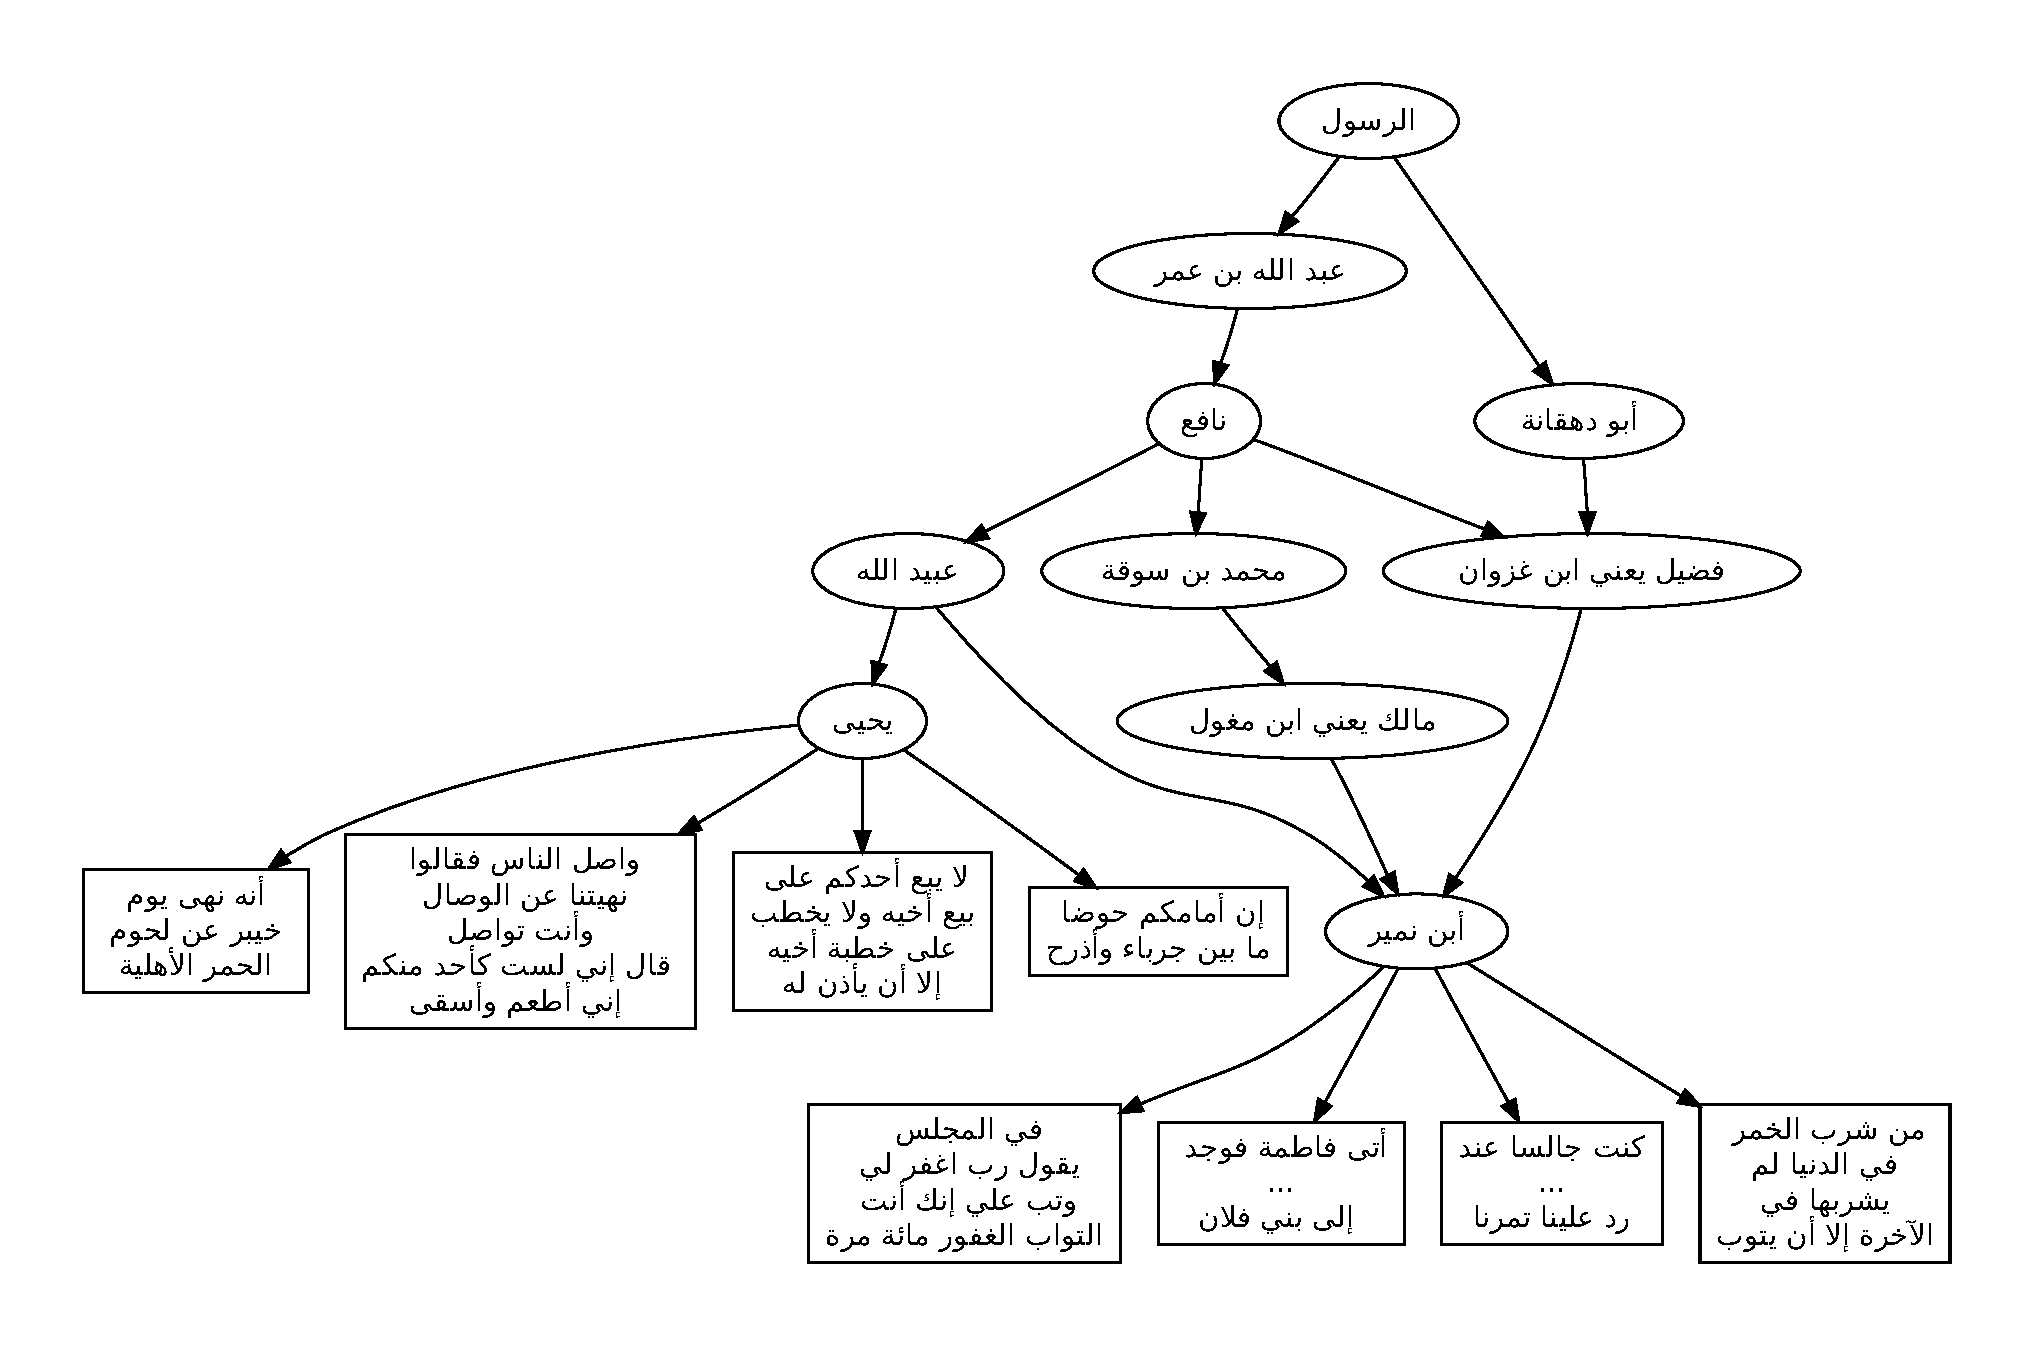
\includegraphics{figs/narrator_chain_output.pdf}}
{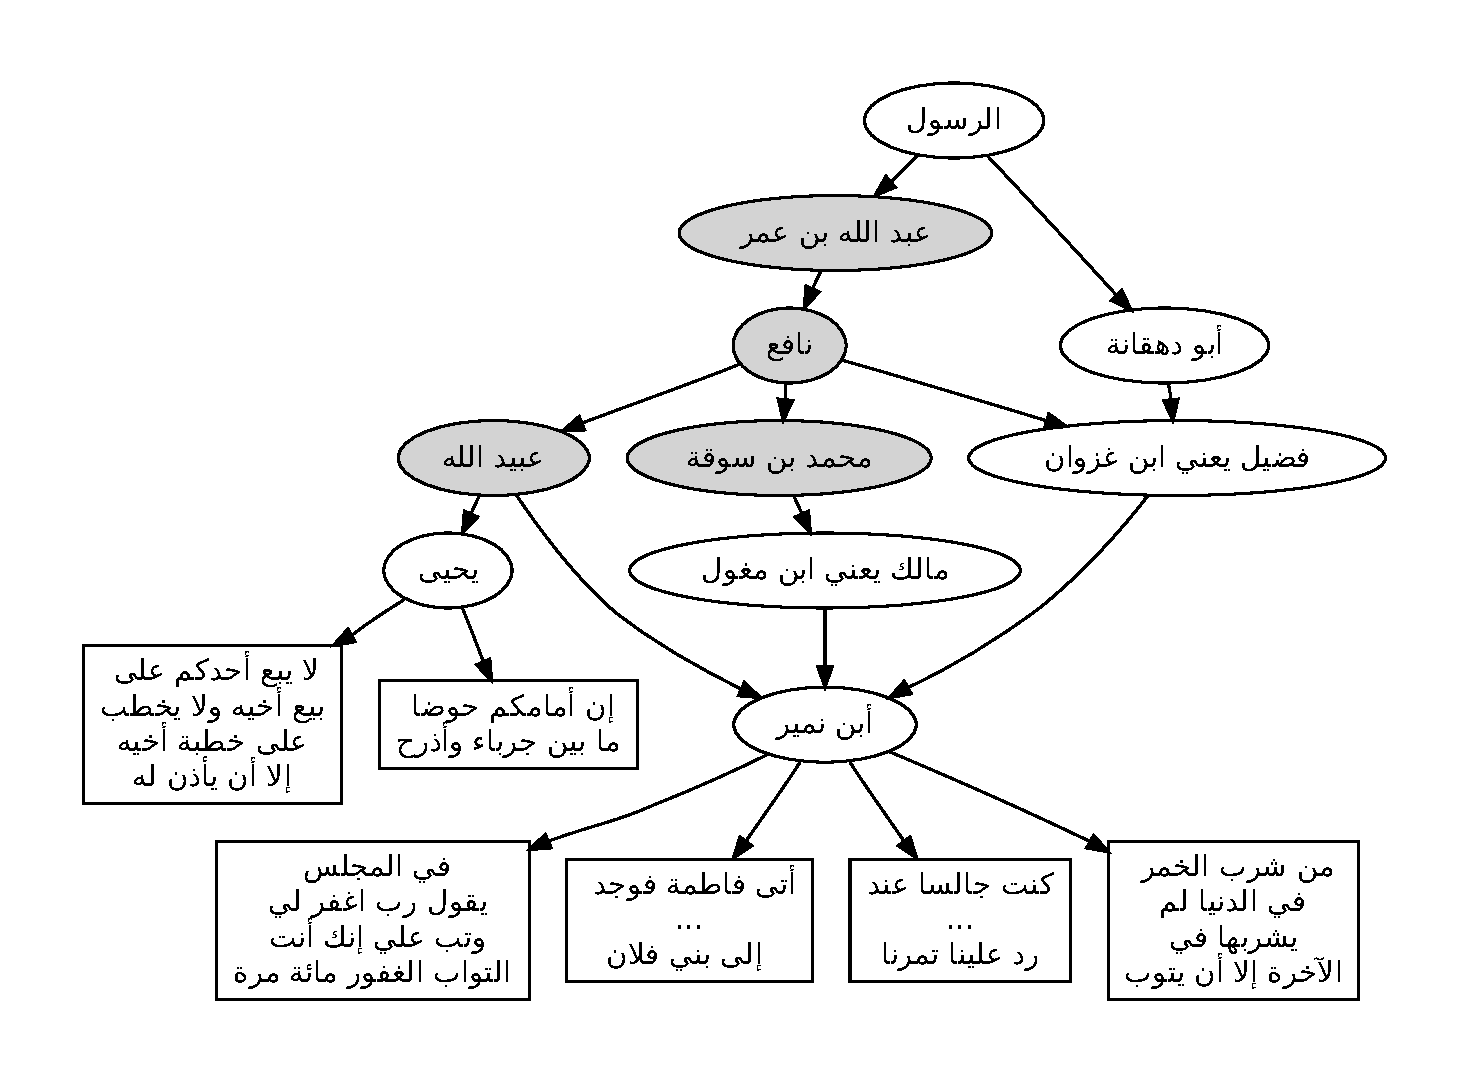
\includegraphics{figs/DAG_narrator.pdf}}
\caption{Narrator directed acyclic graph 
    extracted using NaCEMA }
\label{f:narrators} 
}
\end{figure}

The directed acyclic graph (DAG) 
in Figure~\ref{f:narrators} shows a partial order relation (POR) 
between narrators.
We automatically extracted the POR from the three books of 
hadith~\cite{IbnHanbal,AlKulayni,AlTousi}.
The nodes in boxes are the \RL{matn} of the hadith, 
and the other nodes are the narrators.
Given a set of chains of narrators similar to 
Figure~\ref{f:exhadith} we formed the DAG using graph algorithms 
that merged equal names in the chains. 
We compared the narrators together using a morphological
distance function. 
We considered each narrator to have several morphological 
components and we rewarded every morphological match with 
a small $\delta$. 
Then we applied a threshold $\tau$ to the sum of rewards
and decided the equality of the narrators. 
We omitted the details of the distance function for brevity; 
%
in all cases, we are considering their revisit and re-implementation
in ways more suitable to the hadith case study.

\subsection{Accuracy Results}

\begin{table}[bt]
\centering
\caption{Results of the hadith case study with Sarf.}
%\begin{tabular}{|p{1.5cm}||c|c||c|c||c|c|} \hline
\resizebox{1.1\columnwidth}{!}{
\begin{tabular}{lcp{.2cm}cp{.2cm}c} %\cline{2-10}
 &  AlKafi & & AlIstibsar & &IbnHanbal \\ \cline{1-6}
Word count  &98,943 & & 103,835 & & 20,354 \\ 
 Names       & 12,060  & & 14,613& & 3,013\\
%Names/Narrator & 1.97 & & 1.84& & 1.25 \\
Narrators  & 2,623 & & 5,767& & 1,755 \\ 
%Narrators/Chain  & 4.84 & & 4.76 & &4.05 \\
Chains  & 542 &  & 1,211& & 433 \\ 
Ignored names  & 6,400 &  & 3,348 & & 642 \\ \hline
Segmentation accuracy  & 96\%& & 96\%& & 92\%\\ 
Chain accuracy & 99\%&  & 99\%& & 97\% \\ 
%Narrator accuracy  & & & & &  & & & \\ 
Narrator accuracy  & 91\%& & 90\% & & 90\% \\ \hline
%Name false positives  & 7\%&  & 4\% & & 4\% \\ \hline
Running time (secs.)& 1.32 & & 1.31 & & .096\\ \hline 
\end{tabular}
}
\normalsize
\label{t:hadithresallresults}
\end{table}

We ran our experiments using a dual core 2.66 Ghz 64-bit processor 
with 4GB of memory using a Linux operating system. 
We report our results in Table~\ref{t:hadithresallresults} on the 
three hadith books.
NaCEMA detected narrator chains and segmented the books 
correctly with a chain accuracy above 97\% and a narrator name
accuracy above 90\%
in all cases and across all the 1986 traditions in the three 
different books with different formats. 

The row ``word count'' is an indicator of the size of the data.
The %numbers in 
rows ``names'', ``narrators'', and ``chains'' denote the total
number of the corresponding entities per book.
The row ``ignored names'' reports the number of names detected 
outside the chains and thus are irrelevant to
the application. 
%In addition, the rows ``names/narrator'' and ``narrators/chain'' 
%report the average
%number of names per narrator and 
%the average number of narrators per chain respectively. 

The ``segmentation accuracy'' reports on the accuracy of 
segmentation of the book into separate hadiths.
We computed the metric manually by marking the beginning 
and end of a representative sample of hadiths in each 
book and compared that to the NaCEMA results. 
We used the same approach to compute all other accuracy measures.
The ``chain accuracy'' reflects the percentage of correct narrators 
covered by extracted chains.
The ``narrator name accuracy'' row reflects the percentage of 
correct proper names detected within
narrator structures.

%The row ``name false positives'' reports the percentage of words 
%recognized as names while they should not.
%We notice that this metric did not affect the accuracy
%of narrator and chain segmentation since detecting
%a narrator or a chain with the refined analysis without substantially affecting the 
%high abstract measures such as chain and segmentation
%accuracy.

%\subsection{Future Suggestions}

Although our results reflect a high accuracy, we plan to 
enhance the accuracy of hadith detection and the 
narrator merging algorithms. We also plan to make use of the name connector and narrator
connector stop phrases that our case study extracted to create a 
learning system that can learn more names. 
%We also plan on developing an Arabic linguistic computational model 
%similar to that of ElixirFM~\cite{Otakar:07} but that can be 
%explored partially based on the case study. 

\chapter{Thesis Plan}

The main tasks of the thesis are listed below: \\
\begin{enumerate}[1)]
\item \textbf{Build and Enhance Sarf}
	\begin{enumerate}[\ref*{s:intro}.1)]
	\item Port Buckwalter into C++ and mysql
	\item Implement the Finite State Automata Framework
	\item Implement an application-specific controller interface
	\item Support for disambiguation using diacritics
	\item Support for multi-word expressions
	\item Solve the Issue of `run-on' words
	\item Optimize performance
	\item Support for Running Sarf Under the Windows Operating System
	\item Refactor the code
	\item Write a user Manual
	\item Write a developer manual and documentation
	\end{enumerate}
\item \textbf{Build a time entity extraction application}
\item \textbf{Automate the Hadith Authentication Case Study}
	\begin{enumerate}[3.1)]
	\item Extend the Lexicon of Buckwalter with proper names 
	\item Implement the hadith segmentation tool
	\item Write the Narrator Equality Function
	\item Build Parial Order Graphs
	\item Correct Graph mistakes that result from Ambiguous narrator names which introduce false cycles to the graph
	\item Segment biography books using a graph coloring algorithm
	\item Extract Annotations from the Biography books
	\item Assign annotations to graph nodes
	\item Perform time and possibly location consistency checks
	\item Perform Experiments on the effects of different narrators in Hadith Literature
	\item Write a user Manual
	\item Distribute the tool to willing religious scientists and report their findings
	\end{enumerate}
\item \textbf{Write thesis Report and defend the thesis}
\end{enumerate}

\section{Time Table}

We anticipate that the work can be performed according to the time table presented in
Table~\ref{t:timetable}. \\

~\\

\begin{table}[bt]
\centering
\caption{Thesis Time Table}
\resizebox{1\columnwidth}{!}{
\begin{tabular}{|c|c||c|c||c|c||c||c|c|c|c||c|c|c|c||c|} \bottomrule[0.1em]
\textbf{Year} & \multicolumn{9}{|c|}{\textbf{2011}} & \multicolumn{6}{|c|}{\textbf{2012}} \\ \hline
\textbf{Semester} & ~ & \multicolumn{2}{|c||}{\textbf{\tiny Spring}} & \multicolumn{2}{|c||}{\textbf{\tiny Summer}} 
		& ~ & \multicolumn{4}{|c||}{\textbf{\tiny Fall}} & \multicolumn{4}{|c||}{\textbf{ \tiny Spring}} & ~ \\ \hline
\backslashbox{Task}{Month}
			& \textbf{Done} & \textbf{5} & \textbf{6} & \textbf{7} & \textbf{8} & \textbf{9} & \textbf{\small 10} & 
			 \textbf{\small 11} & \textbf{\small 12} &
			 \textbf{1} & \textbf{2} & \textbf{3} & \textbf{4} & \textbf{5} &
				\begin{tabular}{c}
				\textbf{\small Future} \\
				\textbf{\small Work}
				\end{tabular}
			 \\ \toprule[0.1em] \bottomrule[0.1em]
\textbf{1.1)} & \X & ~ & ~ & ~ & ~ & ~ & ~ & ~ & ~ & ~ & ~ & ~ & ~ & ~ & \\ \hline
\textbf{1.2)} & \X & ~ & ~ & ~ & ~ & ~ & ~ & ~ & ~ & ~ & ~ & ~ & ~ & ~ &\\ \hline
\textbf{1.3)} & \X & ~ & ~ & ~ & ~ & ~ & ~ & ~ & ~ & ~ & ~ & ~ & ~ & ~ & \\ \hline
\textbf{1.4)} & \X & ~ & ~ & ~ & ~ & ~ & ~ & ~ & ~ & ~ & ~ & ~ & ~  & ~ &\\ \hline
\textbf{1.5)} & \X & ~ & ~ & ~ & ~ & ~ & ~ & ~ & ~ & ~ & ~ & ~ & ~ & ~ & \\ \hline
\textbf{1.6)} & \X & ~ & ~ & ~ & ~ & ~ & ~ & ~ & ~ & ~ & ~ & ~ & ~  & ~ &\\ \hline
\textbf{1.7)} & \X & ~ & ~ & ~ & ~ & ~ & ~ & ~ & ~ & ~ & ~ & ~ & ~ & ~ & \\ \hline
\textbf{1.8)} & \x & \X & ~ & ~ & ~ & ~ & ~ & ~ & ~ & ~ & ~ & ~ & ~ & ~ &\\ \hline
\textbf{1.9)} & ~ & ~ & ~ & ~ & ~ & ~ & ~ & ~ & ~ & ~ & ~ & \X & \X & ~ & \\ \hline
\textbf{1.10)}& ~ & ~ & ~ & ~ & ~ & ~ & ~ & ~ & ~ & ~ & ~ & ~ & \X  & ~ & \\ \hline
\textbf{1.11)}& ~ & ~ & ~ & ~ & ~ & ~ & ~ & ~ & ~ & ~ & ~ & ~ & \X & ~ & \\ \toprule[0.1em] \bottomrule[0.1em]
\textbf{2)}   & ~ & ~ & \X & \X & ~ & ~ & ~ & ~ & ~ & ~ & ~ & ~ & ~ & ~ & \\ \toprule[0.1em] \bottomrule[0.1em]
\textbf{3.1)} & \X & ~ & ~ & ~ & ~ & ~ & ~ & ~ & ~ & ~ & ~ & ~ & ~ & ~ & \\ \hline
\textbf{3.2)} & \x & ~ & ~ & ~ & \X & ~ & ~ & ~ & ~ & ~ & ~ & ~ & ~ & ~ & \\ \hline
\textbf{3.3)} & \x & ~ & ~ & ~ & \X & ~ & ~ & ~ & ~ & ~ & ~ & ~ & ~ & ~ & \\ \hline
\textbf{3.4)} & \X & ~ & ~ & ~ & ~ & ~ & ~ & ~ & ~ & ~ & ~ & ~ & ~ & ~ & \\ \hline
\textbf{3.5)} & ~ & ~ & ~ & \X & \X & ~ & ~ & ~ & ~ & ~ & ~ & ~ & ~ & ~ & \\ \hline
\textbf{3.6)} & ~ & ~ & ~ & \X & \X & ~ & ~ & ~ & ~ & ~ & ~ & ~ & ~ & ~ & \\ \hline
\textbf{3.7)} & ~ & ~ & ~ & ~ & ~ & \X & \X & \X & ~ & ~ & ~ & ~ & ~ & ~ & \\ \hline
\textbf{3.8)} & ~ & ~ & ~ & ~ & ~ & ~ & ~ & \X & ~ & ~ & ~ & ~ & ~ & ~ & \\ \hline
\textbf{3.9)} & ~ & ~ & ~ & ~ & ~ & ~ & ~ & ~ & \X & \X & \X & ~ & ~ & ~ & \X \\ \hline
\textbf{3.10)} & ~ & ~ & ~ & ~ & ~ & ~ & ~ & ~ & ~ & ~ & \X & \X & ~ & ~ & \X \\ \hline
\textbf{3.11)} & ~ & ~ & ~ & ~ & ~ & ~ & ~ & ~ & ~ & ~ & ~ & ~ & \X & ~ & \\ \hline
\textbf{3.12)} & ~ & ~ & ~ & ~ & ~ & ~ & ~ & ~ & ~ & ~ & ~ & ~ & ~ & ~ & \X \\ \toprule[0.1em] \bottomrule[0.1em]
\textbf{4)} & ~ & ~ & ~ & ~ & ~ & ~ & ~ & ~ & ~ & ~ & ~ & ~ & ~ & \X &  \\ \hline
\end{tabular}
}
\normalsize
\label{t:timetable}
\end{table}

\large\underline{\textbf{Important Dates}}\\\\
\normalsize
The important dates are as follows:
\begin{itemize}
\item \textbf{Comprehensive exam:} Mid May 2011
\item\textbf{Thesis defense:} Mid May 2012
\end{itemize}

% Include Bibliography
\bibliographystyle{IEEEtran}
{\small \bibliography{jm}}
%\nocite{*}

\end{document}
%-------END----------------------------------------------------
